\providecommand{\toplevelprefix}{../..}  %
\documentclass[../../book-main_ro.tex]{subfiles}

\begin{document}

\chapter{Învățarea Structurilor Liniare și Independente}
\label{ch:classic}\label{ch:linear-independent}

\begin{quote}
\hfill  ``{\em Arta de a face matematică constă în a găsi acel caz special care conține toate germenele generalității}.''


$~$\hfill -- David Hilbert
\end{quote}
\vspace{5mm}







\textit{Datele reale au structură cu dimensiune redusă.} Pentru a vedea de ce acest lucru este adevărat, să considerăm cazul nepretențios al paraziților pe un televizor când satelitul nu funcționează. La fiecare cadru (aproximativ la fiecare \(\frac{1}{30}\) secunde), paraziții RGB pe un ecran de dimensiune \(H \times W\) sunt, aproximativ, eșantionați independent dintr-o distribuție uniformă pe \([0, 1]^{3 \times H \times W}\). În teorie, paraziții \textit{ar putea} să se rezolve într-o imagine naturală la orice cadru dat, dar chiar dacă petreceți o mie de ani uitându-vă la ecranul televizorului, nu se va întâmpla. Această discrepanță este explicată de faptul că setul de imagini naturale \(H \times W\) ocupă o fracțiune dispărut de mică din hipercubul \([0, 1]^{3 \times H \times W}\). În particular, este extrem de mic-dimensional, comparativ cu dimensiunea spațiului ambiental. Fenomene similare apar pentru toate celelalte tipuri de date naturale, cum ar fi text, audio și video. Astfel, când proiectăm sisteme și metode pentru a procesa date naturale și a învăța structura sau distribuția lor, aceasta este o proprietate centrală a datelor naturale pe care trebuie să o luăm în considerare. %

Prin urmare, sarcina noastră centrală este să învățăm o distribuție care are dimensiune intrinsecă redusă într-un spațiu cu dimensiune mare. În restul acestei secțiuni, discutăm câteva metode \textit{clasice} pentru a îndeplini această sarcină pentru câteva modele oarecum {\em idealiste} pentru distribuție, și anume modele care sunt geometric liniare sau statistic independente. Deși aceste modele și metode sunt importante și utile în sine, le discutăm aici deoarece motivează, inspiră și servesc ca un predecesor sau analog pentru metode mai moderne pentru distribuții mai generale care implică învățare profundă (de reprezentare).

Abordarea noastră principală (și formularea generală a problemei) poate fi rezumată ca:
\begin{tcolorbox}\centering
    \textbf{Problemă:} \textit{Având una sau mai multe observații (zgomotoase sau incomplete) ale unui eșantion de adevăr de bază din distribuția datelor, obțineți o estimare a acestui eșantion.}
\end{tcolorbox}
Această abordare stă la baza mai multor metode clasice pentru procesarea datelor, pe care le discutăm în acest capitol.
\begin{itemize}
    \item \Cref{sec:lowrank} --- Analiza Componentelor Principale (PCA): Având eșantioane zgomotoase dintr-o distribuție susținută pe {\em un subspațiu cu dimensiune redusă}, obțineți o estimare a eșantionului adevărat care se află pe acest subspațiu.
    \item  \Cref{sec:ica} --- Învățarea Completă a Dicționarului și Analiza Componentelor Independente (ICA): Având eșantioane zgomotoase dintr-o distribuție susținută pe {\em o reuniune (\textit{nu} extensia) a câtorva subspații cu dimensiune redusă}, obțineți o estimare a eșantioanelor adevărate.
    \item \Cref{sec:dictionary_learning} --- Codificare Rară și Învățarea Dicționarului Supracomplet: Având eșantioane zgomotoase din {\em o distribuție susținută pe combinații de câțiva vectori incoerenți}, cum ar fi axele de coordonate, obțineți o estimare a eșantionului adevărat, care are și această proprietate.
\end{itemize}
După cum vom dezvălui curând în capitolele ulterioare, în era învățării profunde, metodele moderne adoptă în esență aceeași abordare pentru a învăța.

În acest capitol, așa cum s-a descris mai sus, facem ipoteze simplificatoare de modelare care presupun în esență că datele au structuri geometric (aproape, pe bucăți) liniare și componente statistic independente. În \Cref{ch:intro}, ne-am referit la astfel de modele ale datelor ca „modele analitice". Aceste ipoteze de modelare ne permit să derivăm algoritmi eficienți cu garanții de eficiență demonstrabile\footnote{Atât în ceea ce privește complexitatea datelor, cât și cea computațională.} pentru procesarea datelor la scară. Cu toate acestea, ele sunt modele imperfecte pentru distribuțiile de date din lumea reală, adesea complexe, și astfel ipotezele lor fundamentale sunt valabile doar aproximativ. Aceasta înseamnă că garanțiile oferite de analiza detaliată a acestor algoritmi sunt și ele valabile doar aproximativ în cazul datelor reale. Cu toate acestea, tehnicile discutate în acest capitol sunt utile în sine și, dincolo de asta, servesc drept „cazul special cu germenele generalității", ca să spunem așa, în sensul că prezintă o motivație și intuiție ghidatoare pentru paradigmele mai generale din învățarea (profundă) a distribuțiilor mai generale pe care le abordăm ulterior. %






\section{Un Subspațiu cu Dimensiune Redusă} \label{sec:lowrank}

\subsection{Analiza Componentelor Principale (PCA)}\label{sub:pca}

Poate cea mai simplă ipoteză de modelare posibilă pentru structură cu dimensiune redusă
este așa-numita ipoteză de \textit{rang redus}. Lăsând \(D\) să fie dimensiunea
spațiului nostru de date, presupunem că datele noastre aparțin unui subspațiu cu dimensiune redusă de dimensiune \(d \ll D\), posibil plus unele perturbări mici. Aceasta ajunge să fie o ipoteză aproape validă pentru unele date surprinzător de complexe, cum ar fi imagini cu cifre scrise de mână și date faciale \cite{BasriR2003-PAMI} așa cum se arată în \Cref{fig:faces-digits}, totuși, după cum vom vedea, se va preta extrem de bine la o analiză cuprinzătoare.

\begin{figure}
    \centering
    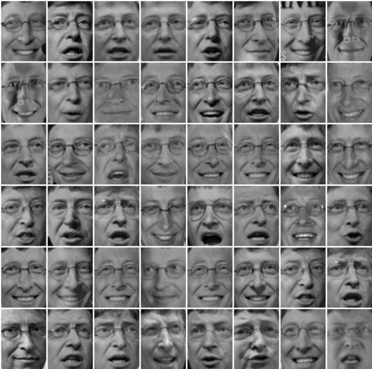
\includegraphics[width=0.4\linewidth]{\toplevelprefix/chapters/chapter2/figs/faces.png}
    \hspace{5mm} 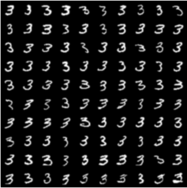
\includegraphics[width=0.395\linewidth]{\toplevelprefix/chapters/chapter2/figs/handwritten-digits.png}   
    \caption{Imagini cu fețe umane și cifre scrise de mână. În ciuda varietății aparent mari în aparențele lor, fiecare set de aceste date acoperă (aproximativ) un subspațiu (aproape) liniar cu dimensiune foarte redusă.}
    \label{fig:faces-digits}
\end{figure}

\paragraph{Formularea problemei.}
Pentru a scrie aceasta în notație matematică, reprezentăm un subspațiu \(\cS \subseteq \R^{D}\) de dimensiune \(d\) printr-o matrice ortonormală \(\vU \in \O(D, d) \subseteq \R^{D \times d}\) astfel încât coloanele lui \(\vU\) să acopere \(\cS\). Apoi, spunem că datele noastre \(\{\vx_{i}\}_{i = 1}^{N} \subseteq \R^{D}\) au structură de rang redus (aproximativ) dacă există o matrice ortonormală \(\vU \in \O(D, d)\), vectori \(\{\vz_{i}\}_{i = 1}^{N} \subseteq \R^{d}\), și vectori \textit{mici} \(\{\veps_{i}\}_{i = 1}^{N} \subseteq \R^{D}\) astfel încât 
\begin{equation}\label{eq:pca_dgp}
    \vx_{i} = \vU\vz_{i} + \veps_{i}, \quad \forall i \in [N].
\end{equation}
Aici \(\veps_{i}\) sunt perturbări care împiedică datele să fie perfect
de rang redus; prezența lor în modelul nostru ne permite să cuantificăm gradul în care
analiza noastră rămâne relevantă în prezența abaterilor de la modelul nostru. Subspațiul
suport adevărat este \(\cS \doteq \mathop{\mathrm{col}}(\vU)\), extensia
coloanelor lui $\vU$. Pentru a procesa tot ce putem din
aceste date, trebuie să recuperăm \(\cS\); pentru a face aceasta este suficient să recuperăm
\(\vU\), numite și \textit{componentele principale}. Din fericire, aceasta este
o sarcină tractabilă computațional numită {\bf Analiza Componentelor Principale}, și
discutăm acum cum să o rezolvăm.

Având date \(\{\vx_{i}\}_{i = 1}^{N}\) distribuite ca în \eqref{eq:pca_dgp}, ne
propunem să recuperăm modelul \(\vU\). O abordare naturală este să găsim subspațiul
\(\vU^{\star}\) și vectorii latenți \(\{\vz_{i}^{\star}\}_{i = 1}^{N}\) care
dau cea mai bună aproximare \(\vx_{i} \approx \vU^{\star}\vz_{i}^{\star}\). Și anume, ne propunem să rezolvăm problema 
\begin{equation}\label{eq:pca_sparse_recovery_problem}
    \min_{\tilde{\vU}, \{\tilde{\vz}_{i}\}_{i = 1}^{N}}\frac{1}{N}\sum_{i = 1}^{N}\norm{\vx_{i} - \tilde{\vU}\tilde{\vz}_{i}}_{2}^{2},
\end{equation}
unde $\tilde{\vU}$ este constrâns să fie o matrice ortonormală, ca mai sus. Vom omite
această constrângere în afirmații similare de mai jos pentru concizie.

\paragraph{Codificare-decodificare subspațiu prin denoising.}
Pentru a simplifica această problemă, pentru un \(\tilde{\vU}\) fixat, avem (demonstrație ca exercițiu):
\begin{align}
    \min_{\{\tilde{\vz}_{i}\}_{i = 1}^{N}}\frac{1}{N}\sum_{i = 1}^{N}\norm{\vx_{i} - \tilde{\vU}\tilde{\vz}_{i}}_{2}^{2} 
    &= \frac{1}{N}\sum_{i = 1}^{N}\min_{\tilde{\vz}_{i}}\norm{\vx_{i} - \tilde{\vU}\tilde{\vz}_{i}}_{2}^{2} \\
    &= \frac{1}{N}\sum_{i = 1}^{N}\norm{\vx_{i} - \tilde{\vU}\tilde{\vU}^{\top}\vx_{i}}_{2}^{2}. 
\end{align}
Adică, soluția optimă \((\vU^{\star}, \{\vz_{i}^{\star}\}_{i = 1}^{N})\)
la problema de optimizare de mai sus are $\vz_i^{\star} = (\vU^{\star})^\top\vx_i$.

Acum, putem scrie problema de optimizare originală în \(\tilde{\vU}^{\star}\)
și \(\{\tilde{\vz}_{i}\}_{i = 1}^{N}\) ca o problemă de optimizare doar peste
\(\tilde{\vU}\), adică, pentru a obține baza \(\vU^{\star}\) și codurile compacte
\(\{\vz_{i}^{\star}\}_{i = 1}^{N}\) este suficient să rezolvăm oricare dintre următoarele două probleme echivalente:
\begin{equation}\label{eq:pca_equals_denoising}
    \min_{\tilde{\vU}, \{\tilde{\vz}_{i}\}_{i = 1}^{N}}\frac{1}{N}\sum_{i = 1}^{N}\norm{\vx_{i} - \tilde{\vU}\tilde{\vz}_{i}}_{2}^{2} = \min_{\tilde{\vU}}\frac{1}{N}\sum_{i = 1}^{N}\norm{\vx_{i} - \tilde{\vU}\tilde{\vU}^{\top}\vx_{i}}_{2}^{2}.
\end{equation}
Observați că problema din partea dreaptă a \eqref{eq:pca_equals_denoising}
este o problemă de \textit{denoising}: având observații zgomotoase \(\vx_{i}\) ale
datelor de rang redus, ne propunem să găsim copia \textit{fără zgomot} a \(\vx_{i}\), care
sub modelul \eqref{eq:pca_dgp} este $\vU\vz_{i}$. Adică, intrarea denoisată
$\hat{\vx}_i = \vU\vU^\top \vx_i$. Observați că acesta este punctul de pe subspațiu
care este cel mai apropiat de $\vx_i$, așa cum este vizualizat în \Cref{fig:pca-geometry}. Aici prin
rezolvarea problemei echivalente de găsire a celui mai bun subspațiu, parametrizat de
baza învățată \(\vU^{\star}\), învățăm o aproximare a
\textit{denoiser}-ului, adică, matricea de proiecție \(\vU^{\star}(\vU^{\star})^{\top} \approx \vU\vU^{\top}\) care proiectează punctul de date zgomotos $\vx_i$ pe subspațiul \(\cS\). %

\begin{figure}
    \centering
    \begin{tikzpicture}
       \node (zero) at (0, 0) {};
       \node (u1) at (5, 1) {\(\vu_{1}\)};
       \draw[blue, ->, thick] (zero) -- (u1);
       \node[circle, inner sep=1.25pt, fill=red, draw=black] (x) at (3, 1.5) {};
       \node[circle, inner sep=1.25pt, fill=green, draw=black] (x_hat) at (3.2, 0.64)  {};
       \node at ($(x) + (0.5, 0.0)$) {\(\vx\)};
       \node at ($(x_hat) + (1, -0.2)$) {\(\hat{\vx} = \vu_{1}\vu_{1}^{\top}\vx\)};
       \draw[brown, ->, thick] (x_hat) -- (x);
       \node at (2.75, 1) {\color{brown}\(\varepsilon\)};
    \end{tikzpicture}
    \caption{\small \textbf{Geometria PCA.} Un punct de date $\vx$ (roșu) este proiectat pe subspațiul unidimensional învățat acoperit de vectorul bază unitar $\vu_1$ (săgeată albastră). Proiecția $\vU\vU^\top\vx = \vu_{1}\vu_{1}^{\top}\vx$ (verde) este versiunea denoisată a $\vx$ folosind structura cu dimensiune redusă dată de $\vu_{1}$, și $\boldsymbol{\varepsilon}$ (săgeată maro) reprezintă reziduul de proiecție sau zgomotul.}
    \label{fig:pca-geometry}
\end{figure}

Punând împreună procesul de mai sus, obținem în esență o schemă simplă de codificare-decodificare care mapează un punct de date $\vx$ în $\R^D$ către un spațiu (latent) cu dimensiune mai mică $\R^d$ și apoi înapoi la $\R^D$:
\begin{equation}
\x \xrightarrow{\hspace{2mm} \mathcal{E} = (\vU^\star)^\top \hspace{2mm}}  \z
    \xrightarrow{\hspace{2mm} \mathcal{D} = \vU^\star \hspace{2mm}}   \hat{\x}.  
\label{eqn:autoencoding-PCA}
\end{equation}
Aici, $\vz \in \R^d$ poate fi văzut ca codul compact cu dimensiune redusă (sau
o reprezentare latentă) a unui punct de date  $\vx \in \R^D$ și baza subspațiului învățat
$\vU^\star$ ca dicționarul asociat ale cărui coloane sunt cuvintele de cod
(învățate) optime. Procesul realizează funcția de denoising a $\vx$ prin
proiectarea lui pe subspațiul acoperit de $\vU^\star$.

\paragraph{Calcularea bazei subspațiului.}
Pentru moment, continuăm calculul nostru. Fie \(\vX = \mat{\vx_{1}, \dots, \vx_{N}} \in \R^{D \times N}\) matricea ale cărei coloane sunt observațiile \(\vx_{i}\). Avem (demonstrație ca exercițiu)
\begin{align}
    \argmin_{\tilde{\vU}}\frac{1}{N}\sum_{i = 1}^{N}\norm{\vx_{i} - \tilde{\vU}\tilde{\vU}^{\top}\vx_{i}}_{2}^{2}
    &= \argmax_{\tilde{\vU}}\frac{1}{N}\sum_{i = 1}^{N}\norm{\tilde{\vU}^{\top}\vx_{i}}_{F}^{2} \\ 
    &= \argmax_{\tilde{\vU}}\tr\rc{\tilde{\vU}^{\top}\bp{\frac{\vX\vX^{\top}}{N}}\tilde{\vU}}.
\end{align}
Astfel, pentru a calcula componentele principale, găsim matricea ortogonală
\(\tilde{\vU}\) care maximizează termenul
\(\tr(\tilde{\vU}^{\top}(\vX\vX^{\top}/N)\tilde{\vU})\). Putem demonstra prin
inducție că această matrice \(\vU^{\star}\) are coloane care sunt \textit{primii \(d\) vectori proprii unitari} ai \(\vX\vX^{\top}/N\). Lăsăm demonstrația întreagă cititorului în \Cref{exercise:principal-components-derivation}, dar tratăm cazul de bază al inducției aici. Să presupunem că \(d = 1\). Atunci avem doar un singur vector unitar \(\vu\) de recuperat, astfel încât problema de mai sus se reduce la
\begin{equation}
    \max_{\tilde{\vu} \colon \norm{\tilde{\vu}}_{2} = 1} \tilde{\vu}^{\top}(\vX\vX^{\top}/N)\tilde{\vu}.
\end{equation}
Acesta este așa-numitul \textit{coeficient Rayleigh} al \(\vX\vX^{\top}/N\). Invocând teorema spectrală diagonalizăm \(\vX\vX^{\top}/N = \vV\vLambda\vV^{\top}\), unde \(\vV\) este ortogonală și \(\vLambda\) este diagonală cu intrări nenagative. Prin urmare 
\begin{equation}
    \tilde{\vu}^{\top}(\vX\vX^{\top}/N)\tilde{\vu} = \tilde{\vu}^{\top}\vV\vLambda\vV^{\top}\vu = (\vV^{\top}\tilde{\vu})^{\top}\vLambda(\vV^{\top}\tilde{\vu}).
\end{equation}
Deoarece \(\vV\) este o transformare ortogonală inversabilă, \(\vV^{\top}\tilde{\vu}\) este un vector unitar, și optimizarea peste \(\tilde{\vu}\) este echivalentă cu optimizarea peste \(\tilde{\vw} \doteq \vV^{\top}\tilde{\vu}\). Prin urmare, putem scrie
\begin{equation}
    \tilde{\vu}^{\top}(\vX\vX^{\top}/N)\tilde{\vu} = \tilde{\vw}^{\top}\vLambda\tilde{\vw},
\end{equation}
ale cărei soluții optime \(\vw^{\star}\) dintre vectorii unitari sunt vectori one-hot a căror singură intrare diferită de zero (deci unitară) este într-unul dintre indicii corespunzători celei mai mari valori proprii a \(\vX\vX^{\top}/N\). Aceasta înseamnă că \(\tilde{\vu} = \vV\tilde{\vw}\), soluția optimă la problema originală, corespunde unui vector propriu unitar al \(\vX\vX^{\top}/N\) (adică, coloană a \(\vV\)) care corespunde celei mai mari valori proprii. Generalizând în mod adecvat aceasta la cazul \(d > 1\), și rezumând toată discuția anterioară, avem următoarea Teoremă informală.
\begin{theorem}\label{thm:pca}
    Să presupunem că setul nostru de date \(\{\vx_{i}\}_{i = 1}^{N} \subseteq \R^{D}\) poate fi scris ca 
    \begin{equation}
        \vx_{i} = \vU\vz_{i} + \veps_{i}, \qquad \forall i \in [N],
    \end{equation}
    unde \(\vU \in \O(D, d)\) captează \textit{structura de rang redus},
    \(\{\vz_{i}\}_{i = 1}^{N} \subseteq \R^{d}\) sunt \textit{codurile compacte}
    ale datelor, și \(\{\veps_{i}\}_{i = 1}^{N} \subseteq \R^{D}\) sunt vectori
    mici care indică abaterea datelor noastre de la modelul de rang redus. Atunci
    \textit{componentele principale} \(\vU^{\star} \in \O(D, d)\) ale setului
    nostru de date sunt date de primii \(d\) vectori proprii ai \(\vX\vX^{\top}/N\),
    unde \(\vX = [\vx_{1}, \dots, \vx_{N}] \in \R^{D \times N}\), și
    corespund aproximativ denoiser-ului liniar optim:
    \(\vU^{\star}(\vU^{\star})^{\top} \approx \vU\vU^{\top}\).
\end{theorem}
Nu dăm rate explicite de aproximare aici deoarece pot deveni destul de
tehnice. În cazul special că \(\veps_{i} = \vzero\) pentru toți \(i\),
\(\vU^{\star}\) învățat acoperă suportul eșantioanelor \(\{\vx_{i}\}_{i
= 1}^{N}\). Dacă în plus \(\vz_{i}\) sunt suficient de diverse (să zicem,
acoperind tot \(\R^{d}\)) atunci am avea recuperare perfectă:
\(\vU^{\star}(\vU^{\star})^{\top} = \vU\vU^{\top}\).

\begin{remark}
    În unele sarcini de analiză a datelor, matricea de date \(\vX\) este formatată astfel încât fiecare punct de date este un \textit{rând} mai degrabă decât o \textit{coloană} așa cum este prezentat aici. În acest caz, componentele principale sunt primii \(d\) vectori proprii ai \(\vX^{\top}\vX/N\).
\end{remark}

\begin{remark}[Selecția Bazei prin Valorile Proprii de Denoising]
    În multe cazuri, fie datele noastre nu vor fi cu adevărat distribuite conform unui model subspațiu-plus-zgomot, fie nu vom cunoaște dimensiunea adevărată de bază \(d\) a subspațiului. În acest caz, trebuie să alegem \(d\); această problemă se numește \textit{selecție de model}. În cazul restrâns al PCA, o modalitate de a efectua selecția modelului este să calculăm \(\vX\vX^{\top}/N\) și să căutăm cazuri în care valorile proprii adiacente scad brusc; acesta este un indicator că indicele valorii proprii mai mari este „dimensiunea adevărată \(d\)", și restul valorilor proprii ale \(\vX\vX^{\top}/N\) sunt contribuite de zgomot sau perturbări \(\veps_{i}\). Selecția modelului este o problemă dificilă și, în zilele noastre în era învățării profunde unde se numește „optimizarea hiperparametrilor", se face de obicei prin forță brută sau optimizare Bayesiană. %
\end{remark}

\begin{remark}[Denoising-ul Eșantioanelor]
    Expresia din partea dreaptă a \eqref{eq:pca_equals_denoising}, adică,
    \begin{equation}\label{eq:orthogonal_denoising}
        \min_{\tilde{\vU}}\frac{1}{N}\sum_{i = 1}^{N}\norm{\vx_{i} - \tilde{\vU}\tilde{\vU}^{\top}\vx_{i}}_{2}^{2},
    \end{equation}
    este ceea ce se numește o problemă de \textit{denoising}, numită astfel deoarece este o problemă de optimizare a cărei soluție \textit{elimină zgomotul din eșantioane astfel încât să se potrivească pe subspațiu}. Denoising-ul---învățarea unei funcții care elimină zgomotul din eșantioane zgomotoase astfel încât să se potrivească pe structura datelor (cum ar fi în \eqref{eq:pca_dgp}, dar poate mai complicat)---este o metodă comună pentru învățarea distribuțiilor care va fi discutată în continuare și pe parcursul manuscrisului. Observați că am discutat deja această noțiune, dar merită repetată datorită importanței sale centrale în capitolele ulterioare.
\end{remark}

\begin{remark}[Interpretarea prin Rețele Neuronale]
    Dacă facem o PCA, recuperăm aproximativ suportul distribuției
    codificat de parametrul \(\vU^{\star}\). Funcția de denoising învățată ia apoi
    forma \(\vU^{\star}(\vU^{\star})^{\top}\). Pe lângă faptul că este
    un denoiser, aceasta poate fi văzută ca o \textit{rețea neuronală liniară simplă
    cu două straturi cu ponderile legate}: primul strat înmulțește cu
    \((\vU^{\star})^{\top}\), și al doilea strat înmulțește cu \(\vU^{\star}\), și anume
    \begin{equation}
        \operatorname{denoise}(\vx) = \underbrace{\vU^{\star} \circ
        \underbrace{\id \circ \underbrace{(\vU^{\star})^{\top}\vx}_{\text{primul ``strat''}}}_{\text{post-activare a primului ``strat''}}}_{\text{ieșirea ``NN''}}
    \end{equation}
    Contrastând aceasta cu o rețea neuronală standard cu două straturi, vedem o similaritate structurală:
    \begin{equation}
        \operatorname{NN}(\vx) = \underbrace{\vW^{\star} \circ
        \underbrace{\mathrm{ReLU} \circ \underbrace{(\vU^{\star})^{\top}\vx}_{\text{primul strat}}}_{\text{post-activare a primului strat}}}_{\text{ieșirea NN}}
    \end{equation}
    În particular, PCA poate fi interpretat ca \textit{învățarea unui autoencoder
    de denoising simplu cu două straturi},\footnote{De fapt, așa cum am menționat în
    capitolul anterior, PCA a fost una dintre primele probleme pe care rețelele neuronale
    au fost folosite pentru a le rezolva \cite{Oja1982SimplifiedNM,Baldi89}.} unul dintre cele mai simple
    exemple de rețea neuronală non-trivială. În acest cadru,
    \textit{reprezentările învățate} ar fi doar \((\vU^{\star})^{\top}\vx \approx \vz\). În acest fel, PCA servește ca o problemă model pentru învățarea (profundă) a reprezentărilor, pe care o vom dezvolta în continuare în monografie. Observați că în această analogie, reprezentările reflectă, sau sunt proiecții ale, datelor de intrare către o structură cu dimensiune redusă învățată. Această proprietate va fi deosebit de relevantă în viitor.
\end{remark}

\subsection{Urmărirea Structurii de Rang Redus prin Iterația Puterii}\label{subsec:power iterations}

Există o modalitate eficientă din punct de vedere computațional de a estima primii vectori proprii ai \(\vX\vX^{\top}/N\) sau orice matrice simetrică pozitiv semidefinită \(\vM\), numită \textit{iterația puterii}. Această metodă este blocul de construcție al mai multor abordări algoritmice pentru analiza datelor cu dimensiune mare pe care le discutăm mai târziu în capitol, așa că o discutăm aici.

Fie \(\vM\) o matrice simetrică pozitiv semidefinită. Există o bază ortonormală pentru \(\R^{D}\) constând din vectori proprii \((\vw_{i})_{i = 1}^{D}\) ai \(\vM\), cu valorile proprii corespunzătoare \(\lambda_{1} \geq \cdots \geq \lambda_{D} \geq 0\). Prin definiție, orice vector propriu $\vw_i$ satisface $\lambda_i \vw_i = \vM \vw_i$. Prin urmare, pentru orice $\lambda_i > 0$, $\vw_i$ este un „punct fix" la următoarea ecuație:
\begin{equation}
    \vw = \frac{\vM\vw}{\norm{\vM\vw}_{2}}.
    \label{eqn:PCA-fixed-point}
\end{equation}

\begin{theorem}[Iterația Puterii]
Presupunem că \(\lambda_{1} > \lambda_{i}\) pentru toți \(i > 1\). Dacă calculăm punctul fix al \eqref{eqn:PCA-fixed-point} folosind următoarea iterație:
\begin{equation}\label{eq:power_iteration}
    \vv_{0} \sim \dNorm(\vzero, \vone), \qquad \vv_{t + 1} \gets \frac{\vM\vv_{t}}{\norm{\vM\vv_{t}}_{2}},
\end{equation}
atunci, în limită, \(\vv_{t}\) va converge către un vector propriu unitar principal al \(\vM\).
\end{theorem}

\begin{proof} În primul rând, observați că pentru toți \(t\), avem 
\begin{equation}
    \vv_{t} = \frac{\vM\vv_{t - 1}}{\norm{\vM\vv_{t - 1}}_{2}} = \frac{\vM^{2}\vv_{t - 2}}{\norm{\vM\vv_{t - 1}}_{2}\norm{\vM\vv_{t - 2}}_{2}} = \cdots = \frac{\vM^{t}\vv_{0}}{\prod_{s = 1}^{t}\norm{\vM\vv_{s}}_{2}}.
\end{equation}
Astfel, \(\vv_{t}\) are aceeași direcție ca \(\vM^{t}\vv_{0}\) și este de normă unitară, astfel încât putem scrie 
\begin{equation}
    \vv_{t} = \frac{\vM^{t}\vv_{0}}{\norm{\vM^{t}\vv_{0}}_{2}}.
\end{equation}
Deoarece toți vectorii proprii \(\vw_{i}\) ai $\vM$ formează o bază ortonormală pentru \(\R^{D}\), putem scrie 
\begin{equation}
    \vv_{0} = \sum_{i = 1}^{D}\alpha_{i}\vw_{i},
\end{equation}
unde deoarece \(\vv_{0}\) este Gaussian, \(\alpha_{i}\) sunt toți diferit de zero cu probabilitate \(1\). Astfel, putem folosi expresia noastră anterioară pentru \(\vv_{t}\) pentru a scrie
\begin{equation}
    \vv_{t} = \frac{\vM^{t}\vv_{0}}{\norm{\vM^{t}\vv_{0}}_{2}} = \frac{\sum_{i = 1}^{D}\lambda_{i}^{t}\alpha_{i}\vw_{i}}{\norm{\sum_{i = 1}^{D}\lambda_{i}^{t}\alpha_{i}\vw_{i}}_{2}} = \frac{\sum_{i = 1}^{D}\lambda_{i}^{t}\alpha_{i}\vw_{i}}{\sum_{i = 1}^{D}\lambda_{i}^{t}\abs{\alpha_{i}}}. 
\end{equation}
Acum, să considerăm cazul în care \(\lambda_{1} > \lambda_{2} \geq \cdots \geq \lambda_{D} \geq 0\). (Cazul cu valori proprii principale repetate merge similar.) Atunci putem scrie
\begin{equation}
    \vv_{t} = \frac{\alpha_{1}\vw_{1} + \sum_{i = 2}^{D}(\lambda_{i}/\lambda_{1})^{t}\alpha_{i}\vw_{i}}{\abs{\alpha_{1}} + \sum_{i = 2}^{D}(\lambda_{i}/\lambda_{1})^{t}\abs{\alpha_{i}}}.
\end{equation}
Deoarece \(\lambda_{1} > \lambda_{i}\) pentru toți \(i > 1\), termenii din interiorul sumei merg la \(0\) exponențial rapid, și restul este limita 
\begin{equation}
    \lim_{t \to \infty}\vv_{t} = \frac{\alpha_{1}}{\abs{\alpha_{1}}}\vw_{1} = \sign(\alpha_{1})\vw_{1},
\end{equation}
care este un vector propriu unitar principal al \(\vM\). Valoarea proprie principală \(\lambda_{1}\) a \(\vM\) poate fi estimată prin \(\vv_{t}^{\top}\vM\vv_{t}\), care converge similar de rapid la \(\lambda_{1}\). 
\end{proof}

Pentru a găsi al doilea vector propriu principal, aplicăm algoritmul de iterare a puterii la \(\vM - \lambda_{1}\vv_{1}\vv_{1}^{\top}\), care are vectori proprii \((\vw_{i})_{i = 2}^{D}\) și valorile proprii corespunzătoare \((\lambda_{i})_{i = 2}^{D}\). Repetând această procedură de \(d\) ori în secvență, putem estima foarte eficient primii \(d\) vectori proprii ai \(\vM\) pentru orice matrice simetrică pozitiv semidefinită \(\vM\). Astfel putem aplica și la \(\vX\vX^{\top}/N\) pentru a recupera primele \(d\) componente principale, ceea ce urmăream de la început. Observați că această abordare recuperează o componentă principală la un moment dat; vom contrasta aceasta cu alte abordări algoritmice, cum ar fi coborârea gradientului pe funcții obiectiv globale, în secțiunile viitoare.




\subsection{PCA Probabilistică}\label{subsec:probabilistic PCA}

Observați că formularea de mai sus nu face ipoteze statistice asupra
procesului de generare a datelor. Cu toate acestea, este obișnuit să includem elemente statistice
într-un model de date dat, deoarece poate adăuga interpretări suplimentare iluminatoare
despre rezultatul analizei. Ca atare, punem întrebarea naturală:
\textit{care este analogul statistic al structurii cu dimensiune redusă?} Răspunsul nostru este că o \textit{distribuție} cu dimensiune redusă este una al cărei suport este concentrat în jurul unei structuri geometrice cu dimensiune redusă.

Pentru a ilustra acest punct, discutăm \textit{analiza componentelor principale probabilistică (PPCA).} Această formulare poate fi văzută ca o variantă statistică a PCA obișnuită. Matematic, considerăm acum datele noastre ca eșantioane dintr-o variabilă aleatoare \(\vx\) care ia valori în \(\R^{D}\) (numită uneori și \textit{vector aleator}). Spunem că \(\vx\) are structură statistică de rang redus (aproximativ) dacă și numai dacă există o matrice ortonormală \(\vU \in \O(D, d)\), o variabilă aleatoare \(\vz\) care ia valori în \(\R^{d}\), și o variabilă aleatoare \textit{mică} \(\veps\) care ia valori în \(\R^{D}\) astfel încât \(\vz\) și \(\veps\) sunt independente, și
\begin{equation}
    \vx = \vU\vz + \veps.
\end{equation}
Scopul nostru este din nou să recuperăm \(\vU\). În acest sens, configurăm problema analogă ca în \Cref{sub:pca}, adică, optimizând peste suporturile subspațiului \(\tilde{\vU}\) și variabilele aleatoare \(\vz\) pentru a rezolva următoarea problemă:
\begin{equation}
    \min_{\tilde{\vU}, \tilde{\vz}}\Ex\norm{\vx - \tilde{\vU}\tilde{\vz}}_{2}^{2}.
\end{equation}
Deoarece găsim cea mai bună astfel de variabilă aleatoare \(\vz\) putem găsi realizarea sa \(\vz(\vx)\) separat pentru fiecare valoare a \(\vx\). Efectuând aceleași calcule ca în \Cref{sub:pca}, obținem %
\begin{equation}\label{eq:ppca_denoising}
    \min_{\tilde{\vU}, \tilde{\vz}}\Ex\norm{\vx - \tilde{\vU}\tilde{\vz}}_{2}^{2} = \min_{\tilde{\vU}}\Ex\min_{\tilde{\vz}(\vx)}\norm{\vx - \tilde{\vU}\tilde{\vz}(\vx)}_{2}^{2} = \min_{\tilde{\vU}}\Ex\norm{\vx - \tilde{\vU}\tilde{\vU}^{\top}\vx}_{2}^{2},
\end{equation}
subliniind din nou faptul că subspațiul estimat cu componentele principale \(\vU^{\star}\) corespunde unui denoiser \(\vU^{\star}(\vU^{\star})^{\top}\) care proiectează pe acel subspațiu. Ca înainte, obținem 
\begin{align}\label{eq:PPCA}
    \argmin_{\tilde{\vU}}\Ex\norm{\vx - \tilde{\vU}\tilde{\vU}^{\top}\vx}_{2}^{2} 
    &= \argmax_{\tilde{\vU}}\Ex\norm{\tilde{\vU}^{\top}\vx}_{2}^{2} \\
    &= \argmax_{\tilde{\vU}}\tr(\tilde{\vU}^{\top}\Ex[\vx\vx^{\top}]\tilde{\vU}),
\end{align}
și soluția la ultima problemă este doar primele \(d\) componente principale ale matricei de moment de ordinul doi \(\Ex[\vx\vx^{\top}]\). De fapt, problemele de mai sus sunt vizual foarte similare cu ecuațiile pentru calcularea componentelor principale din subsecțiunea anterioară, cu excepția că \(\Ex[\vx\vx^{\top}]\) înlocuiește \(\vX\vX^{\top}/N\). De fapt, ultima cantitate este o estimare pentru prima. Ambele formulări fac efectiv același lucru și au aceeași soluție practică---calculați vectorii singulari stângi ai matricei de date \(\vX\), sau echivalent primii vectori proprii ai matricei de covarianță estimate \(\vX\vX^{\top}/N\). Formularea statistică, însă, are o interpretare suplimentară. Să presupunem că \(\Ex[\vz] = \vzero\) și \(\Ex[\veps] = \vzero\). Avem
\begin{equation}
    \Ex[\vx] = \vU\Ex[\vz] + \Ex[\veps] = \vzero,
\end{equation}
astfel încât \(\Cov[\vx] = \Ex[\vx\vx^{\top}]\). Acum calculând \(\Cov[\vx]\) avem 
\begin{equation}
    \Cov[\vx] = \vU\Cov[\vz]\vU^{\top} + \Cov[\veps] = \vU\Ex[\vz\vz^{\top}]\vU^{\top} + \Cov[\veps].
\end{equation}
În particular, dacă \(\Cov[\veps]\) este mic, rezultă că \(\Cov[\vx] = \Ex[\vx\vx^{\top}]\) este aproximativ o matrice de rang redus, în particular rangul \(d\). Astfel primii \(d\) vectori proprii ai \(\Ex[\vx\vx^{\top}]\) rezumă în esență întreaga matrice de covarianță. Dar ei sunt și componentele principale, astfel încât putem interpreta analiza componentelor principale ca efectuând o descompunere de rang redus a \(\Cov[\vx]\).

\begin{remark}
    Folosind punctul de vedere probabilistic al PCA, obținem o înțelegere mai clară și mai cantitativă a modului în care se leagă de denoising. În primul rând, luați în considerare problema de denoising din \eqref{eq:ppca_denoising}, și anume
    \begin{equation}
        \min_{\tilde{\vU}}\Ex\norm{\vx - \tilde{\vU}\tilde{\vU}^{\top}\vx}_{2}^{2}.
    \end{equation}
    Nu este prea greu să demonstrăm că dacă $\tilde{\vU}$ are $d$ coloane și dacă
    \(\veps\) este o variabilă aleatoare Gaussiană izotropă, adică cu distribuție \(\veps \sim \dNorm(\vzero,
    \sigma^{2}\vI)\),\footnote{Alte distribuții funcționează atât timp cât suportă
    tot \(\R^{D}\), dar Gaussiana este cea mai ușor de lucrat aici.} atunci
    pentru \textit{orice} soluție optimă
    \(\vU^{\star}\) la această problemă, avem 
    \begin{equation}
        \vU^{\star}(\vU^{\star})^{\top} = \vU\vU^{\top}
    \end{equation}
    și astfel subspațiul suport adevărat, să zicem \(\cS \doteq \mathop{\mathrm{col}}(\vU)\), este
    recuperat ca extensia coloanelor lui \(\vU^{\star}\), deoarece 
    \begin{equation}
        \cS = \mathop{\mathrm{col}}(\vU) = \mathop{\mathrm{col}}(\vU\vU^{\top})
        = \mathop{\mathrm{col}}(\vU^{\star}(\vU^{\star})^{\top})
        = \mathop{\mathrm{col}}(\vU^{\star}).
    \end{equation}
    În particular, \textit{funcția de denoising} învățată \(\vU^{\star}(\vU^{\star})^{\top}\) este o proiecție ortogonală pe \(\cS\), împingând punctele zgomotoase pe subspațiul suport de adevăr. Putem stabili un rezultat tehnic similar în cazul în care avem doar eșantioane finite, ca în \Cref{thm:pca}, dar aceasta necesită mai mult efort și tehnicitate. Rezumând această discuție, avem următoarea Teoremă informală.
\end{remark}


\begin{theorem}\label{thm:ppca}
    Să presupunem că variabila aleatoare \(\vx\) poate fi scrisă ca
    \begin{equation}
        \vx = \vU\vz + \veps
    \end{equation}
    unde \(\vU \in \O(D, d)\) captează \textit{structura de rang redus}, \(\vz\)
    este un vector aleator care ia valori în \(\R^{d}\), și \(\veps\) este un vector
    aleator care ia valori în \(\R^{D}\) astfel încât \(\vz\) și \(\veps\) sunt
    independente, și \(\veps\) este mic. Atunci \textit{componentele principale}
    \(\vU^{\star} \in \O(D, d)\) ale setului nostru de date sunt date de primii \(d\)
    vectori proprii ai \(\Ex[\vx\vx^{\top}]\), și corespund aproximativ
    denoiser-ului liniar optim: \(\vU^{\star}(\vU^{\star})^{\top} \approx \vU\vU^{\top}\).
\end{theorem}



\subsection{Completarea Matricei}

În subsecțiunile anterioare, am discutat problema \textit{învățării unei distribuții geometrice sau statistice de rang redus}, unde datele au fost eșantionate dintr-un subspațiu cu zgomot aditiv. Dar aceasta nu este singurul tip de perturbare dintr-o distribuție cu dimensiune redusă care merită studiat. În această subsecțiune, introducem încă o clasă de erori non-aditive care devin din ce în ce mai importante în învățarea profundă. Să considerăm cazul în care avem unele date \(\{\vx_{i}\}_{i = 1}^{N}\) generate conform \eqref{eq:pca_dgp}. Acum le aranjăm într-o matrice \(\vX = \mat{\vx_{1}, \dots, \vx_{N}} \in \R^{D \times N}\). Spre deosebire de înainte, nu observăm \(\vX\) direct; în schimb ne imaginăm că observația noastră a fost coruptă pe drum și am obținut 
\begin{equation}
    \vY = \vM \hada \vX,
\end{equation}
unde \(\vM \in \{0, 1\}^{D \times N}\) este o \textit{mască} care este cunoscută de noi,
și \(\hada\) este înmulțirea element cu element. În acest caz, scopul nostru este să recuperăm \(\vX\) (de unde putem folosi PCA pentru a recupera \(\vU\), etc), având doar observația coruptă \(\vY\), masca \(\vM\), și cunoașterea că \(\vX\) este (aproximativ) de rang redus. Aceasta se numește \textit{completarea matricei de rang redus}.

Există multe resurse excelente care discută algoritmi și abordări pentru a rezolva această problemă \cite{Wright-Ma-2022}. Într-adevăr, aceasta și generalizări similare ale acestei probleme de recuperare a structurii de rang redus sunt rezolvate de „PCA robust". Nu vom intra în metoda de soluție aici. În schimb, vom discuta în ce condiții această problemă este \textit{plauzibilă} de rezolvat. Pe de o parte, în cazul cel mai absurd, să presupunem că fiecare intrare a matricei \(\vX\) ar fi aleasă independent de toate celelalte. Atunci nu ar exista nicio speranță de a recupera \(\vX\) exact chiar dacă ar lipsi o singură intrare și am avea \(DN - 1\) intrări. Pe de altă parte, să presupunem că am ști că \(\vX\) are rangul 1 exact, care este o condiție extrem de puternică asupra structurii cu dimensiune redusă a datelor, și ne-am confrunta cu masca
\begin{equation}
    \vM = \mat{\vone_{(D - 1) \times 1} & \vzero_{(D - 1) \times (N - 1)} \\ 1 & \vone_{1 \times (N - 1)} }.
\end{equation}
Atunci știm că datele sunt distribuite pe o linie și cunoaștem un vector pe
acea linie---este doar prima coloană a matricei \(\vY = \vM \hada \vX\). Din ultima coordonată a fiecărei coloane, de asemenea dezvăluită nouă de mască, putem rezolva pentru fiecare coloană deoarece pentru fiecare coordonată finală există un singur vector pe linie cu această coordonată. Astfel putem reconstrui \(\vX\) cu o acuratețe perfectă și avem nevoie doar de un număr liniar de observații \(D + N - 1\).

În lumea reală, problemele reale sunt undeva între cele două cazuri limită discutate mai sus. Cu toate acestea, diferențele dintre aceste două extreme, precum și discuția anterioară despre PCA, dezvăluie un nucleu general de adevăr:
\begin{quote}
    \centering
    \textit{Cu cât distribuția datelor este mai mică dimensional și mai structurată, cu atât este mai ușor de procesat și sunt necesare mai puține observații---cu condiția ca algoritmul să utilizeze eficient această structură cu dimensiune redusă.}
\end{quote}
După cum este poate previzibil, vom întâlni acest motiv în mod repetat în restul manuscrisului, începând chiar în secțiunea următoare.








\section{Un Amestec de Subspații Complete cu Dimensiune Redusă}%
\label{sec:ica}
După cum am văzut, modelele de semnal de rang redus sunt suficient de bogate pentru a oferi o imagine completă a interacțiunii dintre dimensionalitatea redusă în date și algoritmii computaționali eficienți și scalabili pentru reprezentare și recuperare sub erori.
Aceste modele implică o conductă de învățare a reprezentării \textit{liniară} și simetrică \eqref{eqn:autoencoding-PCA}:
\begin{equation*}
    \vz = \cE(\vx) = \vU^\top \vx, \quad \hat{\vx} = \cD(\vz) = \vU \vz,
\end{equation*}
care poate fi învățată demonstrabil din eșantioane finite de $\vx$ cu analiza componentelor principale (rezolvată eficient, să zicem, cu metoda puterii) ori de câte ori distribuția de $\vx$ este cu adevărat liniară.
Aceasta este o ipoteză restrictivă---căci, așa cum Harold Hotelling, distinsul statistician din secolul 20,\footnote{Întâmplător, de asemenea faimos pentru contribuțiile sale la dezvoltarea și denumirea Analizei Componentelor Principale \cite{Hotelling1933}.} a obiectat în urma prezentării teoriei sale de programare liniară de către George Dantzig pentru prima dată \cite{Dantzig2002-eh},
\begin{quote}
\centering
    \textit{``...cu toții știm că lumea este neliniară.''}
\end{quote}


\begin{figure}
    \centering
    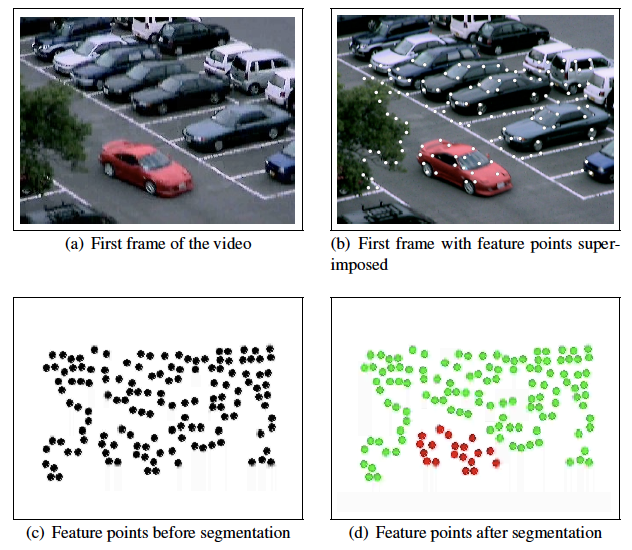
\includegraphics[height=0.35\linewidth]{\toplevelprefix/chapters/chapter2/figs/motion.png} \hspace{5mm}
    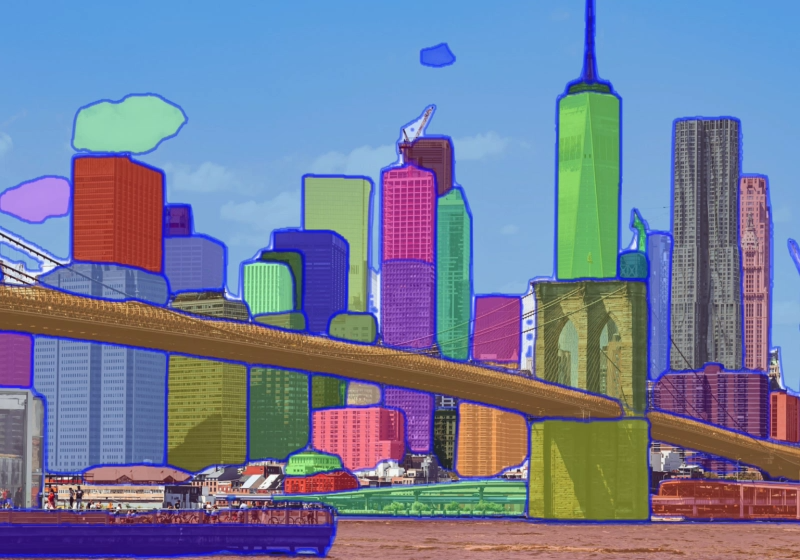
\includegraphics[height=0.349\linewidth]{\toplevelprefix/chapters/chapter2/figs/segment.png} 
    \caption{\textbf{Stânga:} caracteristici urmărite pe obiecte care se mișcă independent într-o scenă. \textbf{Dreapta:} patch-uri de imagine asociate cu diferite regiuni ale unei imagini.}
    \label{fig:multiple-subspaces}
\end{figure}
Chiar ținând cont de eleganța și simplitatea sa, ipoteza de rang redus este prea restrictivă pentru a fi aplicabilă în general la modelarea datelor din lumea reală.
O limitare cheie este ipoteza unui \textit{singur} subspațiu liniar care este responsabil pentru generarea observațiilor structurate.
În multe aplicații practice, structura generată de un \textit{amestec} de
subspații distincte cu dimensiune redusă oferă un model mai realist.
De exemplu, considerați o secvență video care capturează mișcarea mai multor obiecte distincte, fiecare supus propriei deplasări independente (\Cref{fig:multiple-subspaces} stânga).
Sub ipoteze adecvate asupra mișcărilor individuale, fiecare obiect devine responsabil pentru un subspațiu independent cu dimensiune redusă în secvența concatenată de cadre video \cite{VidalR2004-ECCV}.
Ca un alt exemplu, considerați modelarea imaginilor naturale prin învățarea unui model pentru
distribuția \textit{patch-urilor}, colecții contigue spațial de
pixeli, în cadrul unei imagini (\Cref{fig:multiple-subspaces} dreapta). Spre deosebire de
exemplul Eigenface pe care l-am văzut anterior, unde imaginile fețelor cu poze
potrivite pot fi bine aproximate printr-un singur subspațiu cu dimensiune redusă, patch-ul
dintr-o locație specifică dintr-o imagine naturală poate corespunde obiectelor cu
proprietăți foarte diferite---de exemplu, culoare sau formă distinctă din cauza
limitelor de ocluzie. Prin urmare, modelarea distribuției patch-urilor cu un singur
subspațiu este inutilă, dar un \textit{amestec} de subspații, unul pentru fiecare regiune,
funcționează surprinzător de bine în practică, să zicem pentru segmentare sau compresie
\cite{Mobahi-IJCV2011}.\footnote{Vom reveni la această observație în
\Cref{ch:representation}, unde vom arăta că poate fi generalizată semnificativ
pentru a învăța reprezentări pentru seturi de date moderne la scară largă.} Vom vedea un exemplu concret în capitolul următor (\Cref{eg:image-segmentation}).



\begin{figure}
    \centering
    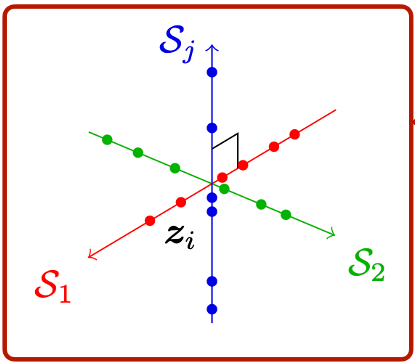
\includegraphics[height=0.35\linewidth]{\toplevelprefix/chapters/chapter2/figs/subspaces.png}
    \caption{Date pe un amestec de subspații cu dimensiune redusă, să zicem $\mathcal{S}_j
    = \mathop{\mathrm{col}}(\vU_j)$.}
    \label{fig:subspaces}
\end{figure}

În această secțiune, vom începe prin a discuta fundamentele conceptuale și algoritmice
pentru învățarea reprezentării structurate când distribuția datelor
poate fi modelată prin {\em un amestec de subspații cu dimensiune redusă}, așa cum este ilustrat în \Cref{fig:subspaces}. În această setare, maparea decodorului va fi aproape la fel de simplă ca în cazul unui singur subspațiu: reprezentăm simplu prin
\begin{equation}\label{eq:mixture-subspaces-decoder-first-cut}
    \hat{\x} = \cD(\vz) = \left( \sum_{k=1}^K \pi_k(\vz)\vU_k \right) \vz,
\end{equation}
unde $\pi_k : \R^d \to \set{0,1}$ sunt un set de variabile aleatoare de ponderare \textit{rare},
astfel încât doar un singur subspațiu $\mathcal{S}_k
= \mathop{\mathrm{col}}(\vU_k) $ este selectat în sumă.
Cu toate acestea, sarcina de a codifica astfel de date $\vx$ în reprezentări adecvate $\vz$, și de a învăța o astfel de pereche codor-decodor din date, se va dovedi a fi mai complexă.

Vom vedea cum ideile din bogata literatură despre \textit{reprezentare rară}
și \textit{analiza componentelor independente} duc la o reformulare naturală a
arhitecturii decodorului de mai sus prin prisma rarității, arhitectura codorului corespunzătoare
(obținută printr-un algoritm de tip metodă a puterii analog
cu cel al analizei componentelor principale), și garanții puternice de corectitudine
și eficiență pentru învățarea unor astfel de perechi codor-decodor din date. În acest sens,
cazul structurii liniare mixte cu dimensiune redusă duce deja la multe dintre
componentele conceptuale cheie ale învățării reprezentării structurate pe care le vom dezvolta în
generalitate mult mai mare în această carte.


\subsection{Amestecuri de Subspații și Dicționare Folosite Rar}\label{sec:mixture-and-dict}


Fie $\vU_1, \dots, \vU_K$, fiecare de dimensiune $D \times d$, să denoteze o colecție de baze ortonormale pentru $K$ subspații de dimensiune $d$ în $\R^D$.
A spune că $\vx$ urmează o distribuție de amestec de subspații parametrizată de $\vU_1, \dots, \vU_K$ înseamnă, geometric vorbind,
că 
\begin{equation}\label{eq:mixture-of-subspaces-geometric}
    \vx = \vU_k \vz  \quad \text{pentru un anumit} \enspace k \in [K],\enspace \vz \in \R^d.
\end{equation}
Analogul statistic al acestui model geometric, așa cum am văzut pentru cazul PCA și al structurii liniare,
este că $\vx$ urmează o distribuție de \textit{amestec de Gaussiene}: adică,
\begin{equation}\label{eq:mixture-of-subspaces-statistical}
    \vx \sim \sum_{k=1}^K \pi_k \cN(\mathbf{0}, \vU_k\vU_k^\top), \quad \text{pentru unele} \enspace \pi_k \geq 0,\enspace \sum_{k=1}^K \pi_k = 1.
\end{equation}
Cu alte cuvinte, pentru fiecare $k \in [K]$, $\vx$ este Gaussian pe subspațiul cu dimensiune redusă
$\mathop{\mathrm{col}}(\vU_k)$ cu probabilitate $\pi_k$.

\begin{remark}[Un Amestec de Gaussiene vs. O Suprapunere de Gaussiene]
Ar trebui să fim conștienți că modelul de mai sus
    \eqref{eq:mixture-of-subspaces-statistical} este un \textit{amestec} de
    distribuții Gaussiene, să nu fie confundat cu un amestec de
    variabile Gaussiene prin suprapunere, să zicem 
\begin{equation}
    \vx = \sum_{i=1}^n w_i \vx_i, \quad \vx_i \sim \cN(\mathbf{0}, \vU_i\vU_i^\top),
\end{equation}
unde $\vx_i$ sunt vectori Gaussieni aleatori independenți și $w_i$ sunt un set de ponderi fixe. După cum știm din proprietățile vectorilor Gaussieni, o astfel de suprapunere $\vx$ va rămâne o distribuție Gaussiană.
\end{remark}

Pentru moment, ne concentrăm pe perspectiva geometrică oferită de \eqref{eq:mixture-of-subspaces-geometric}.
Există o alternativă convenabilă algebric la această reprezentare condiționată. Considerați un vector de reprezentare \textit{ridicat} $\vz = [\vz_1^\top, \dots, \vz_K^\top]^\top \in \R^{dK}$, astfel încât $\vz$ este \textit{$d$-rar} cu suport pe unul dintre cele $K$ blocuri consecutive neîncălecate de $d$ coordonate din $dK$. 
Atunci \eqref{eq:mixture-of-subspaces-geometric} poate fi scris echivalent ca
\begin{equation}\label{eq:mixture-of-subspaces-dictionary-pre}
    \vx = 
    \underbrace{
    \begin{bmatrix} 
    | & \hdots & |  \\
    \vU_1 & \hdots & \vU_K  \\
    | & \hdots & | 
    \end{bmatrix} 
    }_{\vU}
    \underbrace{
    \begin{bmatrix} \vz_1 \\ \vdots \\ \vz_K \end{bmatrix}
    }_{\vz},
    \quad
    \norm*{
    \begin{bmatrix} \norm*{\vz_1}_2 \\ \vdots \\ \norm*{\vz_K}_2 \end{bmatrix}
    }_0 = 1.
\end{equation}
Aici, „norma" $\ell^0$ $\norm{\,\cdot\,}_0$ măsoară raritatea numărând numărul de intrări diferite de zero:
\begin{equation}\label{eq:ell-zero-norm}
    \norm{\vz}_0 = \abs*{\set{i \given z_i \neq 0}},
\end{equation}
și matricea $\vU \in \R^{D \times Kd}$ se numește \textit{dicționar} cu toate $\{\vU_i\}_{i=1}^K$ ca cuvinte de cod. În general, dacă numărul de subspații din amestec $K$ este suficient de mare, nu există o limită a numărului de coloane conținute în dicționarul $\vU$. În cazul în care $Kd < D$, $\vU$ se numește \textit{subcomplet};
când $Kd = D$, se numește \textit{complet}; și când $Kd > D$, se numește \textit{supracomplet}. 

Acum, \eqref{eq:mixture-of-subspaces-dictionary-pre} sugerează o relaxare convenabilă pentru tractabilitatea analizei: în loc să modelăm $\vx$ ca provenind dintr-un amestec de $K$ subspații \textit{specifice} $\vU_1, \dots, \vU_K$, putem începe în schimb cu un dicționar $\vU \in \R^{D \times m}$, unde $m$ poate fi mai mic sau mai mare decât $D$, și pur și simplu căutăm să reprezentăm $\vx = \vU \vz$ cu raritatea $\norm{\vz}_0$ suficient de mică.
Aceasta duce la \textit{modelul de dicționar rar} pentru $\vx$:
\begin{equation}\label{eq:mixture-of-subspaces-dictionary}
    \vx =  \vU \vz + \veps,
    \quad
    \norm{\vz}_0 \ll d,
\end{equation}
unde $\veps$ reprezintă un vector de zgomot necunoscut.
Geometric, aceasta implică că $\vx$ se află aproape de extensia unui subset de $\norm{\vz}_0$ coloane ale $\vU$,
făcând aceasta o instanțiere a modelului de amestec de subspații \eqref{eq:mixture-of-subspaces-geometric} cu o valoare foarte mare a $K$, și corelații specifice între subspațiile $\vU_k$.


\paragraph{Dicționar ortogonal pentru codificare rară.}
Acum putem formula problema de învățare a reprezentării structurate pentru amestecuri de subspații cu dimensiune redusă pe care o vom studia în această secțiune.
Presupunem că avem eșantioane $\vX = [\vx_1, \dots, \vx_N]$ dintr-un model de dicționar rar necunoscut \eqref{eq:mixture-of-subspaces-dictionary}, posibil cu zgomote adăugate $\veps_i$.
Să începem de la ipoteza că dicționarul $\vU$ în modelul de dicționar
rar \eqref{eq:mixture-of-subspaces-dictionary} este complet și
ortogonal,\footnote{Se poate arăta că pentru cazul complet, nu pierdem nicio generalitate făcând ipoteza ortogonală (\Cref{exercise:whitening}).} și că fiecare vector de coeficienți $\vz$ este $d$-rar, cu $d \ll D$.
În această setare, învățarea reprezentării echivalează cu învățarea corectă a dicționarului ortogonal $\vU$ prin optimizare: putem
lua apoi $\cE(\vx) = \vU^\top \vx$ ca encoder și $\cD(\vz) = \vU \vz$
ca decoder, și $\cD = \cE^{-1}$. În formă de diagramă:
\begin{equation}
\vx \xrightarrow{\hspace{2mm} \mathcal{E} = \vU^\top \hspace{2mm}}  \vz \xrightarrow{\hspace{2mm} \mathcal{D} = \vU \hspace{2mm}}   \hat{\vx}.  
\label{eqn:autoencoding-DL}
\end{equation}    
Vedem că perechea de autocodificare $(\cE, \cD)$ pentru învățarea completă a dicționarului este simetrică, ca în cazul unui singur subspațiu liniar, făcând sarcina computațională de codificare și decodificare nu mai dificilă decât în cazul liniar. Pe de altă parte, sarcina de a învăța dicționarul $\vU$ este strict mai dificilă decât învățarea unui singur subspațiu liniar prin PCA.
Pentru a vedea de ce nu putem folosi pur și simplu PCA pentru a învăța corect dicționarul ortogonal $\vU$, observați că 
funcția de pierdere care a dat naștere la PCA, și anume \eqref{eq:pca_equals_denoising}, este
complet invariantă la rotațiile rândurilor matricei $\vU$: adică, dacă
$\vQ$ este orice matrice ortogonală $d \times d$, atunci $\vU$ și $\vU \vQ$ sunt ambele
fezabile și au o pierdere identică pentru \eqref{eq:pca_equals_denoising}.
Modelul de dicționar rar nu este în mod decisiv invariant la astfel de transformări: dacă
am înlocui $\vU$ cu $\vU \vQ$ și am face o rotație corespunzătoare $\vQ^\top \vz$
a coeficienților de reprezentare $\vz$, am distruge în general structura de raritate a $\vz$, încălcând ipoteza de modelare. Astfel, avem nevoie de noi algoritmi pentru învățarea dicționarelor ortogonale.

\subsection{Învățarea Completă a Dicționarului}
\label{sec:complete-dictionary}

În această secțiune, vom deriva algoritmi pentru rezolvarea problemei de învățare a dicționarului ortogonal. Pentru a fi mai preciși, presupunem că vectorul observat $\vx \in \R^D$ urmează un model statistic
\begin{equation}
    \vx = \vU \vz + \veps, 
    \label{eq:ica-model-ch2}
\end{equation}
unde $\vU \in \R^{D \times D}$ este un dicționar ortogonal necunoscut, $\vz$ este un vector aleator cu componente statistic independente $z_i$, fiecare cu medie zero, și $\veps \in \R^D$ este un vector aleator independent de zgomote (Gaussiene) mici. Scopul este să recuperăm $\vU$ (și prin urmare $\vz$) din eșantioane de $\vx$.

Aici presupunem că fiecare componentă independentă $z_i$ este distribuită ca $$z_i \sim \mathrm{Bern}(\theta) \cdot \cN(0, 1/\theta).$$ Adică, este produsul unei variabile aleatoare Bernoulli cu probabilitate $\theta$ de a fi $1$ și $1-\theta$ de a fi $0$, și o variabilă aleatoare Gaussiană independentă cu varianță $1/\theta$. Această distribuție este cunoscută formal ca distribuția {\em Bernoulli-Gaussiană}. 
Normalizarea este aleasă astfel încât $\Var(z_i) = 1$ și prin urmare $\bE[\norm{\vz}_2^2]=d$. 
Această ipoteză de modelare implică că vectorul componentelor independente $\vz$ este de obicei foarte rar: 
calculăm $\bE\left[\norm{\vz}_0\right] = d\theta$, care este mic când $\theta$ este invers proporțional cu $d$. 

\begin{remark}[Ipoteza Ortogonală] 
La prima vedere, ipoteza că dicționarul $\vU$ este ortogonal ar putea părea să fie oarecum restrictivă. Dar de fapt nu există pierdere de generalitate. Se poate considera un dicționar complet ca fiind orice matrice pătrată inversabilă $\vU$. Cu eșantioane generate din acest dicționar: $\vX = \vU \vZ \in \mathbb{R}^{D\times N}$, este ușor de arătat că cu o anumită precondiționare a matricei de date $\vX$: 
\begin{equation}
    \bar{\vX} = \Big(\frac{1}{N\theta} \vX\vX^\top\Big)^{-\frac{1}{2}}\vX,
\end{equation}
atunci există o matrice ortogonală $\vU_{o} \in \O(D)$ astfel încât
\begin{equation}
    \bar{\vX} = \vU_{o}\vZ.
\end{equation}
    Vezi \Cref{exercise:whitening} sau \cite{sun2017completeI} pentru mai multe detalii.
\end{remark}



\begin{figure}
    \centering
    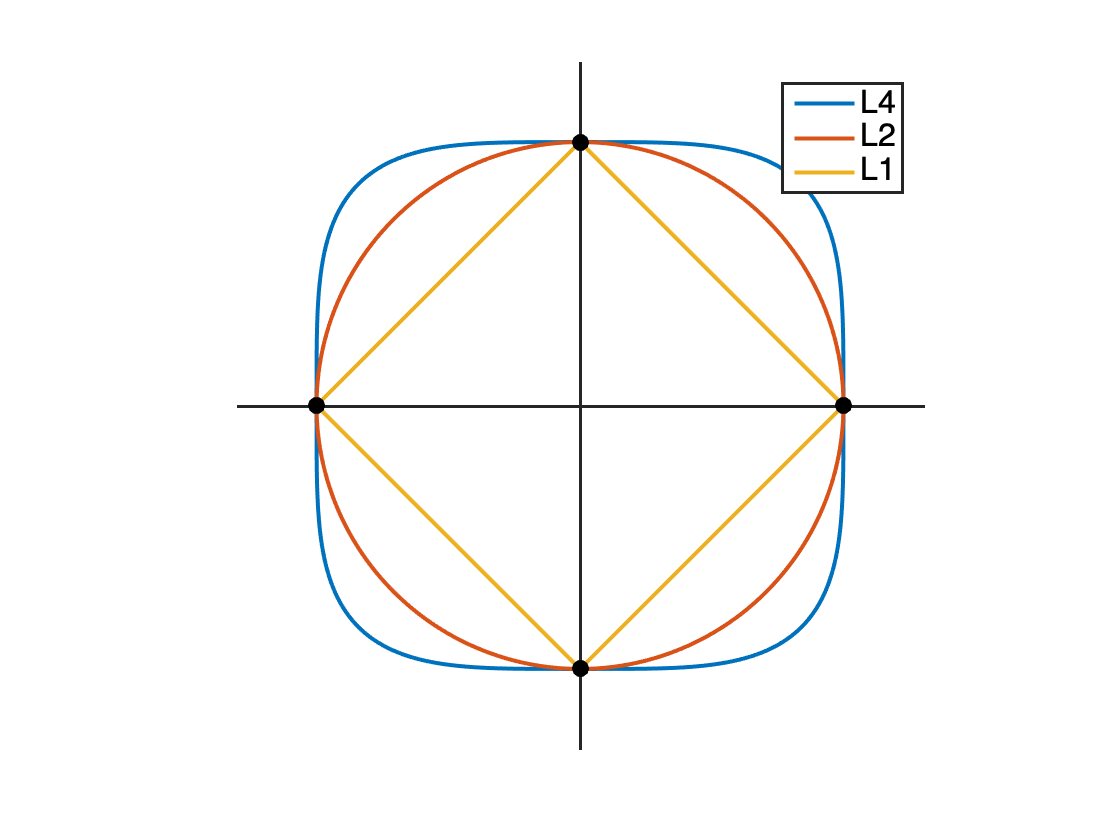
\includegraphics[width=0.6\linewidth]{\toplevelprefix/chapters/chapter2/figs/2DL4Sphere.png}\vspace{-0.1in}
    \caption{Maximizarea normei $\ell^4$ sau minimizarea normei $\ell^1$ promovează raritatea (pentru vectori pe sferă).}
    \label{fig:L4-sphere}
\end{figure}


\paragraph{Învățarea dicționarului prin algoritmul MSP.}

Acum să presupunem că avem un set de observații:
\begin{equation}
    \vx_i = \vU \vz_i + \veps_i,\ \forall i \in [N].
\end{equation}
Fie $\vX = [\vx_1, \dots, \vx_N]$ și $\vZ = [\vz_1, \dots, \vz_N]$. Scopul este să recuperăm $\vU$ din datele $\vX$. Prin urmare, având orice matrice ortogonală $\vA \in \O(D)$, 
\begin{equation}
    \vA\vx_i = \vA\vU \vz_i + \vA\veps_i
\end{equation}
ar fi aproape rară dacă $\vA = \vU^T$ (deoarece prin ipoteză zgomotul $\veps_i$ are magnitudine mică). 

De asemenea, având $\vU$ ortogonal și faptul că $\veps$ este mic, vectorul $\vx$ are o normă așteptată previzibilă, adică $\bE[\norm{\vx}_2^2] \approx \bE[\norm{\vz}_2^2]=d$. Este un fapt cunoscut că pentru vectori pe o sferă, maximizarea normei $\ell^4$ este echivalentă cu minimizarea normei $\ell^0$ (pentru promovarea rarității),
\begin{equation}
    \argmax_{\vz \in \mathbb{S}^n}\|\vz\|_{4}\quad\Leftrightarrow\quad \argmin_{\vz \in \mathbb{S}^n}\|\vz\|_{0}.
\end{equation}
Aceasta este ilustrată în \Cref{fig:L4-sphere}.

O matrice ortogonală $\vA$ păstrează norma Euclidiană (\(\ell^{2}\)): $\|\vA \vx\|_2^2 = \|\vx\|_2^2$. Prin urmare, pentru a găsi dicționarul ortogonal corect $\vU$ din $\vX$, putem încerca să rezolvăm următorul program de optimizare:
\begin{equation}\label{eq0:orthogonal-dictionary-learning-l4}
    \max_{\tilde{\vA} \in \O(D)}\,
     \frac{1}{4} \norm*{
    \tilde{\vA} \vX
    }_4^4 =  \frac{1}{4} \sum_{i=1}^N \norm*{
        \tilde{\vA} \vx_i
    }_4^4
\end{equation}
Aceasta este cunoscută ca problema de maximizare $\ell^4$ \cite{Zhai-2020}. După ce
găsim soluția \(\vA^{\star}\), putem lua transpusa \(\vU^{\star}
= (\vA^{\star})^{\top}\).
\begin{remark}
    Este de asemenea cunoscut că pentru vectori pe o sferă, minimizarea normei $\ell^1$ este echivalentă cu minimizarea normei $\ell^0$ (pentru promovarea rarității),
\begin{equation*}
            \argmin_{\vz \in \mathbb{S}^n}\|\vz\|_{1}\quad\Leftrightarrow\quad \argmin_{\vz \in \mathbb{S}^n}\|\vz\|_{0},
\end{equation*}
care este de asemenea ilustrată în \Cref{fig:L4-sphere}. Acest fapt poate fi de asemenea exploatat pentru a învăța dicționarul $\vA$ eficient și eficace. Aceasta a fost de fapt explorată mai devreme decât norma $\ell^4$ folosită aici. Cititorii interesați pot consulta lucrarea \cite{qu2020findingsparsestvectorssubspace}.
\end{remark}

Observați că problema de mai sus este echivalentă cu următoarea problemă de optimizare constrânsă:
\begin{equation}\label{eq:orthogonal-dictionary-learning-l4}
    \min\,
    -   \frac{1}{4} \norm*{
    \tilde{\vA} \vX
    }_4^4 \quad \mbox{cu condiția} \quad  \tilde{\vA}^\top\tilde{\vA} = \vI.
\end{equation}
După cum se arată în \cite{Wright-Ma-2022}, folosind metoda multiplicatorilor Lagrange, se poate deriva că soluția optimă la problemă ar trebui să satisfacă următoarea 
condiție de „punct fix":
\begin{equation}
    \vA^{\star} = \mathcal{P}_{\mathrm O(D)}[( {\vA^{\star} \vX})^{\hada 3}\vX^\top],
\end{equation}
unde $\mathcal{P}_{\mathrm O(D)}[\,\cdot\,]$ este o proiecție pe spațiul
matricelor ortogonale $\mathrm O(D)$.\footnote{Pentru orice matrice $\vM$ cu SVD $\vM = \vU\bm \Sigma \vV^\top$, $\mathcal{P}_{\mathrm O(D)}[\vM] = \vU \vV^\top$. Lăsăm aceasta ca exercițiu pentru cititor.} 

Pentru a calcula punctul fix pentru ecuația de mai sus, similar cu modul în care am calculat
vectorii proprii pentru PCA \eqref{eqn:PCA-fixed-point}, putem lua următoarea
iterație a puterii:
\begin{equation}\label{eq:msp_iteration}
    \vA_{t+1} = \mathcal{P}_{\mathrm O(D)}[( {\vA_t \vX})^{\hada 3}\vX^\top].
\end{equation}
Aceasta este cunoscută ca algoritmul {\em potrivire, întindere și proiecție} (MSP) propus de \cite{Zhai-2020}. S-a demonstrat că în condiții largi un astfel de algoritm greedy converge într-adevăr la soluția corectă la o rată superliniară.

\begin{remark}[Optimalitatea Globală a Maximizării $\ell^4$]\label{rem:L4-global}
Problema de maximizare $\ell^4$ constrânsă este un program neconvex. În general nu ar trebui să ne \textit{așteptăm} ca algoritmi greedy (să zicem de tip gradient descent) să convergă la soluția global optimă. Surprinzător, se poate arăta că, spre deosebire de programele neconvexe generale, peisajul maximizării $\ell^4$ peste o sferă
\begin{equation}\label{eq:l4-maximization-sphere}
    \min\,
    -   \frac{1}{4} \norm*{
    \vq^\top \vX
    }_4^4 \quad \mbox{cu condiția} \quad  \vq^\top\vq = 1.
\end{equation}
este foarte benign: Toate minimele locale sunt aproape de optimele globale și toate punctele critice sunt puncte șa cu o direcție de curbură negativă. Prin urmare, orice metodă de coborâre cu capacitatea de a scăpa de punctele șa stricte găsește demonstrabil soluții global optime. Pentru afirmații mai precise, cititorii interesați pot consulta \cite{Qu2020Geometric}. 
\end{remark}

\begin{remark}[Rețea Liniară Profundă Stabilă]
Procesul iterativ de mai sus de calculare a dicționarului are o interpretare naturală incrementală de „învățare profundă". Să definim 
$\delta \vA_{t+1} = \vA_{t+1}\vA_{t}^\top$ și $\vZ_t = \vA_t \vX$, atunci este ușor de arătat că
$$\delta \vA_{t+1} = \mathcal{P}_{\mathrm O(D)}[(\vZ_t)^{\hada 3} \vZ_t^\top].$$ 
Dacă $\vA_t$ converge la dicționarul corect $\vD_o$, atunci procesul de codificare iterativ de mai sus este în esență echivalent cu o „rețea liniară profundă": 
$$\vZ \; \longleftarrow \; \vZ_{t+1} =  \underbrace{\delta \vA_{t+1} \delta \vA_{t} \ldots \delta \vA_{1}}_{\color{red} \text{straturi construite înainte}} \vX.$$
Observați că calculul transformărilor incrementale $\delta \vA_{t+1}$ la fiecare strat depinde doar de ieșirea caracteristicilor din stratul anterior $\vZ_t$. Rețeaua este natural stabilă deoarece fiecare strat este o transformare ortogonală care păstrează norma. În ciuda asemănării sale cu o rețea liniară profundă, backpropagarea nu este necesară pentru a învăța fiecare strat. Toate straturile sunt învățate într-o singură trecere înainte!
\end{remark}


\subsection{Conexiunea cu ICA și Kurtosis}
Cu modelul Bernoulli-Gaussian, variabilele $z_i$ sunt independente și non-Gaussiene. Atunci, există o corespondență clară între învățarea dicționarului și analiza clasică a componentelor independente (ICA), în măsura în care algoritmii pentru a rezolva o problemă pot fi folosiți pentru a rezolva cealaltă.\footnote{Explorăm această problemă mai în profunzime în \Cref{exercise:symmetry-identifiability}, unde se face o conexiune între non-Gaussianitatea componentelor independente și noțiunea pur geometrică de simetrie. Această problemă este legată de observația noastră de mai sus că PCA nu funcționează pentru recuperarea dicționarelor ortogonale folosite rar: în setarea statistică, poate fi legată de invarianța rotațională a distribuției Gaussiene (\Cref{exercise:gaussian-rot-invar}).} 


Către derivarea unui algoritm bazat pe ICA, ne concentrăm pe o funcție obiectiv cunoscută ca \textit{kurtosis}, care este folosită în ICA ca o consecință directă a non-Gaussianității componentelor. \textit{Kurtosis}, sau cumulantul de ordinul patru, al unei variabile aleatoare $X$ cu medie zero este definit ca
\begin{equation}\label{eq:kurtosis}
\kurt(X) = \Ex{X^4} - 3 (\Ex{X^2})^2.
\end{equation}
Dacă avem doar eșantioane finite din variabila aleatoare $X$ aranjate într-un vector $\vx = [x_1, \dots, x_N]$, definim kurtosis prin media lor empirică, care dă
\begin{equation}\label{eq:kurtosis-vector}
\kurt(\vx) = \frac{1}{N} \norm{\vx}_4^4 - \frac{3}{N^2} \norm{\vx}_2^4.
\end{equation}
În final, pentru vectori aleatori, definim kurtosis-ul lor ca suma kurtosis-ului scalar al fiecărei componente.
Kurtosis este o funcție de pierdere naturală pentru ICA deoarece pentru $X$ Gaussian, kurtosis este zero; cititorul poate verifica în plus că distribuția Bernoulli-Gaussiană are kurtosis pozitiv.
Astfel o procedură naturală pentru căutarea componentelor independente non-Gaussiene este să căutăm un set de direcții mutual-ortogonale $\vV \in \R^{d \times k}$ astfel încât $\vV^\top \vX$ să aibă kurtosis maxim, unde $\vX = \vU \vZ \in \R^{D \times N}$ este matricea de date ICA Bernoulli-Gaussiană.
Formal, căutăm să rezolvăm problema
\begin{equation}
    \max_{\vV^\top \vV = \vI} \kurt(\vV^\top \vX).
\end{equation}
La o extremă, putem seta $k = D$ și căutăm să recuperăm întregul dicționar
$\vU$ dintr-o singură lovitură. Se poate arăta că această problemă poate fi rezolvată cu
algoritmul MSP pe care l-am văzut anterior.
La cealaltă extremă, putem seta $k=1$ și căutăm să recuperăm o singură direcție (coloană a $\vU$) la un moment dat, efectuând \textit{deflație}, adică, înlocuind matricea de date $\vX$ cu $(\vI - \vu\vu^\top) \vX$, după fiecare pas înainte de a găsi o altă direcție.
Există un compromis natural între scalabilitatea abordării incrementale $k=1$ și eficiența și robustețea abordării $k=D$.

\paragraph{ICA incrementală: corectitudine și algoritmul FastICA.}
Algoritmul FastICA, avansat de Hyv\"{a}rinen și Oja \cite{hyvarinen-1997}, este un algoritm rapid cu punct fix pentru rezolvarea schemei de maximizare a kurtosis-ului $k=1$ pentru ICA.
Problema în cauză este
\begin{equation}\label{eq:kurtosis-maximization-sphere-finitesample}
    \max_{\norm{\vv}_2^2 = 1}\, \kurt(\vX^\top \vv).
\end{equation}
În primul rând, vom efectua o analiză foarte de bază a acestui obiectiv pentru a verifica corectitudinea sa. Observați prin schimbarea de variabile $\vw = \vU^\top \vv$ că această problemă este echivalentă cu
\begin{equation*}
    \max_{\norm{\vw}_2^2 = 1}\, 
    \mathrm{kurt}(\vZ^\top \vw).
\end{equation*}
Acest obiectiv este suficient de simplu încât putem face afirmații puternice despre corectitudinea sa ca formulare pentru recuperarea dicționarului $\vU$.
De exemplu, în setarea populației unde $N \to \infty$, 
putem folosi proprietățile de aditivitate ale kurtosis-ului (\Cref{exercise:kurtosis-linearity-properties}) și normalizarea noastră asumată asupra componentelor independente pentru a scrie problema anterioară echivalent ca
\begin{equation}\label{eq:kurtosis-maximization-sphere-population-simple}
    \max_{\norm{\vw}_2^2 = 1}\, 
    \sum_{i=1}^d \mathrm{kurt}(z_i) w_i^4.
\end{equation}
Se poate arăta că sub ipoteza Bernoulli-Gaussiană, peisajul de optimizare al acestei probleme este „benign" (\Cref{exercise:kurtosis-sphere-landscape})---însemnând că toate maximele locale ale funcției obiectiv corespund recuperării uneia dintre componentele independente.
O modalitate eficientă și scalabilă de a calcula unul dintre aceste maxime este prin algoritmi de optimizare de ordinul întâi, care urmează iterativ gradientul funcției obiectiv și proiectează pe setul de constrângeri $\set{\vw \given \norm{\vw}_2^2 = 1}$.
Deoarece am presupus că fiecare $z_i$ satisface $\Var(z_i)=1$, avem 
pentru $N$ mare
\begin{equation}\label{eq:kurtosis-approximation-l4}
    \kurt(\vX^\top \vu)
    \approx
    \tfrac{1}{N} \norm{\vX^\top \vu}_4^4 - 3 \norm{\vu}_2^4.
\end{equation}
Putem deriva apoi o aproximare corespunzătoare a gradientului:
\begin{equation*}
    \nabla_{\vu} \kurt(\vX^\top \vu)
    \approx
    \tfrac{4}{N} \vX (\vX^\top \vu)^{\hada 3}
    - 12 \norm{\vu}_2^2 \vu.
\end{equation*}
Algoritmul FastICA folosește o metodă cu punct fix pentru a calcula direcțiile de kurtosis maxim. Începe de la condițiile de optimalitate de ordinul întâi pentru problema de maximizare a kurtosis-ului, având în vedere aproximarea gradientului precedent și setul de constrângeri, care citesc
\begin{align}\label{eq:kurtosis-max-sphere-stationarity}
   \vX (\vX^\top \vu)^{\hada 3} 
   = 
   \underbrace{
   \ip*{\vu}{
   \vX (\vX^\top \vu)^{\hada 3} 
   }}_{\lambda} \vu,
\end{align}
unde valoarea specifică a $\lambda$ este determinată folosind constrângerea de normă unitară pe $\vu$.
\Cref{exercise:sphere-calculus} descrie fundalul matematic necesar pentru a deriva aceste condiții de optimalitate din principii prime.
Ecuația \eqref{eq:kurtosis-max-sphere-stationarity} este satisfăcută de \textit{orice} punct critic al problemei de maximizare a kurtosis-ului; vrem să derivăm o ecuație satisfăcută doar de maximizatori.
După ce observăm că $\lambda = \norm{\vX^\top \vu}_4^4$, re-exprimăm echivalent \eqref{eq:kurtosis-max-sphere-stationarity} ca ecuația modificată
\begin{align}\label{eq:kurtosis-max-sphere-stationarity-modified}
   \frac{1}{N}\vX (\vX^\top \vu)^{\hada 3} 
   - 
   3 \vu
   = 
   \left(
   \frac{\lambda}{N} - 3
   \right)
   \vu,
\end{align}
și realizăm că orice maximizator al \eqref{eq:kurtosis-maximization-sphere-finitesample} 
trebuie să satisfacă $\lambda / N - 3 > 0$,
presupunând că $N$ este suficient de mare.
Prin urmare, putem \textit{normaliza} ambele părți ale \eqref{eq:kurtosis-max-sphere-stationarity-modified},
dând următoarea ecuație cu punct fix satisfăcută de fiecare maximizator al \eqref{eq:kurtosis-maximization-sphere-finitesample}:
\begin{align}\label{eq:kurtosis-max-sphere-fxp}
\frac{
   \frac{1}{N}\vX (\vX^\top \vu)^{\hada 3} 
   - 
   3 \vu
   }{
   \norm*{
   \frac{1}{N}\vX (\vX^\top \vu)^{\hada 3} 
   - 
   3 \vu
   }_2
   }
   =
   \vu.
\end{align}
Iterând maparea definită de partea stângă a acestei expresii cu punct fix obținem apoi algoritmul FastICA al lui Hyv\"{a}rinen și Oja \cite{hyvarinen-1997}:
\begin{equation}
\begin{split}\label{eq:fast-ica}
   \vv^+ &= \tfrac{1}{N}\vX (\vX^\top \vu)^{\hada 3}- 3 \vu
   ,  \\
   \vu^+ &= \vv^+ / \norm*{\vv^+}_2.
   \end{split}
\end{equation}
Se dovedește că algoritmul FastICA converge extrem de rapid (de fapt la
o rată \textit{cubică}) la coloanele dicționarului $\vU$; cititorii interesați
pot consulta \cite{hyvarinen-1997} pentru detalii. 
Comparând algoritmul FastICA \eqref{eq:fast-ica} cu metoda puterii studiată
în \Cref{sub:pca} pentru problema PCA și algoritmul MSP
\eqref{eq:msp_iteration}, observăm o similaritate izbitoare. Într-adevăr, FastICA este în esență o metodă a puterii modificată, implicând gradientul kurtosis-ului empiric mai degrabă decât gradientul liniar mai simplu al obiectivului PCA.


\section{Un Amestec de Subspații Supracomplete cu Dimensiune Redusă}
\label{sec:dictionary_learning}
După cum am văzut, învățarea completă a dicționarului se bucură de o teorie computațională elegantă în care menținem o structură de autocodificare simetrică $\cE(\vx) = \vU^\top \vx$, $\cD(\vz) = \vU \vz$, cu un algoritm scalabil de tip metodă a puterii (algoritmul MSP) pentru învățarea unui dicționar/carte de coduri ortogonal $\vU$ din date. Cu toate acestea, pentru învățarea reprezentărilor distribuțiilor generale de date cu dimensiune mare, trebuie să extindem dimensiunea cărții de coduri dincolo de cerința ortogonalității---însemnând că trebuie să avem $\vA \in \R^{D \times m}$, cu $m \gg D$, corespunzând cazului unui dicționar/carte de coduri \textit{supracomplet},\footnote{Schimbăm notația aici de la $\vU$ la $\vA$ pentru a sublinia non-ortogonalitatea și forma non-pătrată a dicționarului supracomplet $\vA$.} și modelul de semnal
\begin{equation}\label{eq:model-DL-overcomplete}
    \vx =  \vA \vz + \veps,
    \quad
    \norm{\vz}_0 = d \ll m.
\end{equation}
Există atât motivații geometrice, cât și fizice/de modelare pentru trecerea la cazul supracomplet.
Geometric, amintiți-vă că în reducerea noastră originală de la modelul de date cu amestec de subspații la modelul de dicționar rar, un amestec de $K$ subspații în $\R^D$, fiecare de dimensiune $d$, a dus la un dicționar de formă $\vA \in \R^{D \times Kd}$.
Cu alte cuvinte, dicționarele supracomplete corespund amestecurilor \textit{mai bogate} de subspații, cu mai multe moduri distincte de variabilitate pentru modelarea distribuției de date cu dimensiune mare.
Pe partea de modelare, putem rula un experiment computațional pe date din lumea reală care dezvăluie puterea suplimentară de modelare conferită de o reprezentare supracompletă.

\begin{figure}[t]
\centering
    \begin{subfigure}{0.9\linewidth}
        \centering
        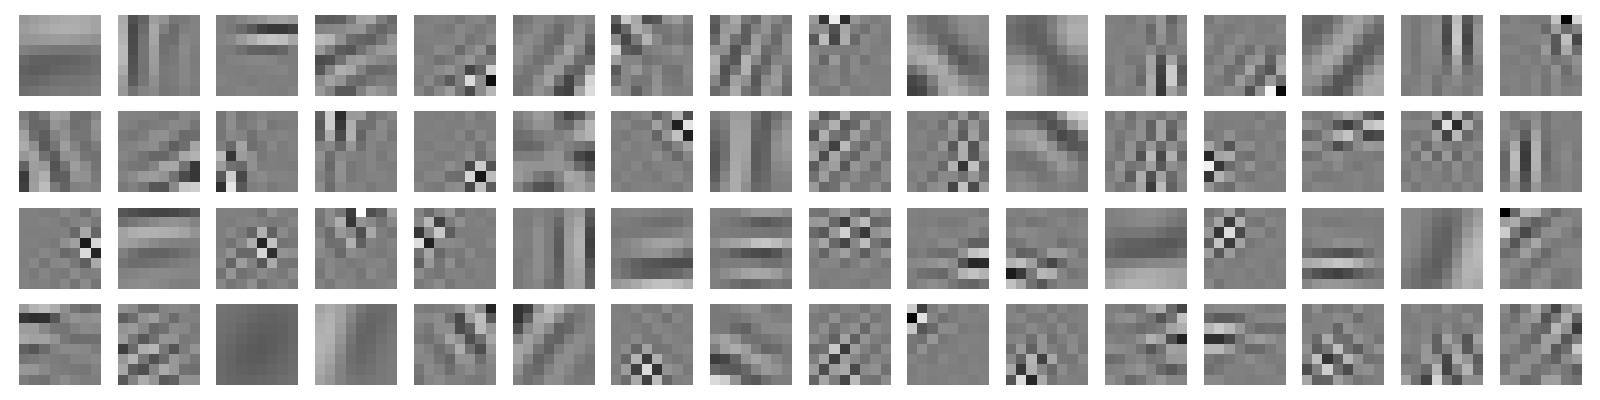
\includegraphics[width=\linewidth]{\toplevelprefix/chapters/chapter2/figs/msp_atoms_patches_new.png}
        \caption{}
    \end{subfigure}
    \begin{subfigure}{0.9\linewidth}
        \centering
        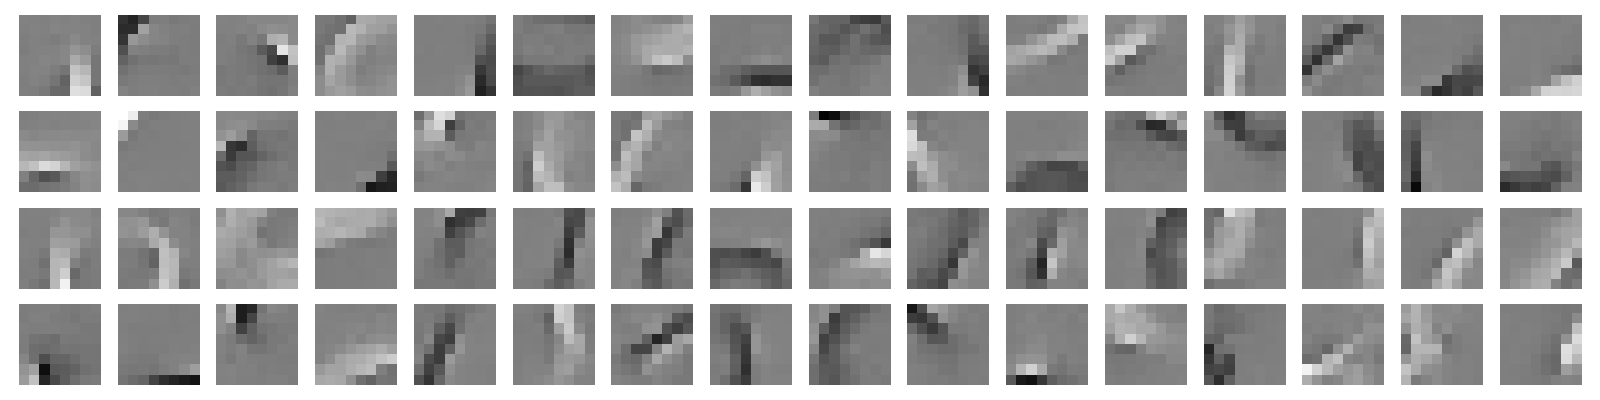
\includegraphics[width=\linewidth]{\toplevelprefix/chapters/chapter2/figs/palm_atoms_patches_new.png}
        \caption{}
    \end{subfigure}
    \caption{Comparație între atomii de dicționar învățați pentru dicționare complete (ortogonale)
    și supracomplete, antrenate pentru a reconstrui patch-uri de $8$ pe $8$ luate din
    cifre MNIST. Ambele dicționare sunt antrenate pentru $6000$ de epoci pe $10^4$ patch-uri aleatorii cu
    conținut netrivial, iar codurile rare sunt calculate cu obiectivul LASSO
    și $\lambda=0.1$ (vezi \eqref{eq:sparse_dl_lasso}). Hărțile de culori au negru pentru valori negative și alb pentru
    valori pozitive. \textbf{Sus:} Un dicționar ortogonal învățat cu
    algoritmul MSP \eqref{eq:msp_iteration} este constrâns să
    aibă nu mai mult de $64$ de atomi; atomii învățați corespund aproximativ unui
    dicționar de tip „spike and slab", și obțin niveluri de raritate de reconstrucție
    relativ slabe pe datele de test nefolosite (codurile sunt aproximativ $17$-rare în
    medie, în raport cu un prag de $10^{-1}$).
    \textbf{Jos:} În contrast, un dicționar supracomplet (aici, cu $8^3$
    atomi; vizualizăm un subset aleator de $64$) învață
    atomi de dicționar semnificativi semantic corespunzând marginilor orientate
    cu semn, care pot fi asamblate pentru a crea patch-uri de cifre și a obține
    niveluri superioare de reconstrucție și raritate. Codurile sunt aproximativ
    $20$-rare în
    medie, fiind de $8$ ori mai mari decât cele ale dicționarului
    ortogonal. Pentru a calcula
    dicționarul, folosim un optimizator bazat pe minimizare alternată linearizată
    proximală pe o versiune regularizată adecvat a
    \eqref{eqn:DL-overcomplete}.}
    \label{fig:ReconMNIST}
\end{figure}

\begin{example}
Având imagini eșantionate de cifre scrise de mână, \Cref{fig:ReconMNIST}(a) arată rezultatul potrivirii unui dicționar ortogonal la setul de date.
În contrast, \Cref{fig:ReconMNIST}(b) arată rezultatul rulării unui
algoritm de optimizare pentru învățarea dicționarelor supracomplete (pe care îl vom
prezenta în detaliu mai târziu în Capitol) pe aceste eșantioane.
Observați că reprezentările devin mult mai rare și cărțile de coduri mult mai interpretabile---ele constau din primitive fundamentale pentru liniile care compun cifrele, adică margini orientate.
\end{example}


De fapt, învățarea dicționarului supracomplet a fost propusă inițial ca un algoritm biologic plauzibil pentru reprezentarea imaginilor bazat pe dovezi empirice despre modul în care etapele timpurii ale cortexului vizual reprezintă stimulii vizuali \cite{Olshausen1996-ap,Olshausen1997-yv}.

În restul acestei secțiuni, vom prezenta fundamentele conceptuale și computaționale ale învățării dicționarului supracomplet.
Presupunând că modelul \eqref{eq:model-DL-overcomplete} este satisfăcut cu
coduri rare \(\vz\), dicționar supracomplet \(\vA\), și nivel de raritate \(d\),
și având eșantioane \(\vX = [\vx_1, \dots, \vx_N]\) de \(\vx\), vrem să învățăm
un encoder \(\cE : \R^D \to \R^m\) mapând fiecare \(\vx\) la {codul său rar}
\(\vz\), și un decoder \(\cD(\vz) = \vA \vz\) reconstruind fiecare \(\vx\) din
codul său rar. %
În formă de diagramă:
\begin{equation}
\x \xrightarrow{\hspace{4mm} \mathcal{E} \hspace{4mm}}  \z \xrightarrow{\hspace{2mm} \mathcal{D} = \vA \hspace{2mm}}   \hat{\x}.  
\label{eqn:autoencoding-DL-overcomplete}
\end{equation}

Vom începe de la construcția encoderului $\cE$.
Vom lucra incremental: mai întâi, \textit{având dicționarul adevărat $\vA$}, vom arăta cum problema de \textit{codificare rară} oferă un algoritm elegant, scalabil și demonstrabil corect pentru recuperarea codului rar $\vz$ al lui $\vx$.
Deși această problemă este NP-hard în cazul cel mai rău, poate fi rezolvată eficient și scalabil pentru dicționare $\vA$ care sunt \textit{incoerente}, adică având coloane care nu sunt prea corelate.
Arhitectura encoderului cuprinsă de această soluție nu va mai fi simetrică: vom vedea că are forma unei rețele profunde primitive, care depinde de dicționarul $\vA$.

Apoi vom proceda la sarcina de a învăța decodorul $\cD$, sau echivalent dicționarul supracomplet $\vA$.
Vom deriva un algoritm pentru învățarea dicționarului supracomplet care ne permite 
să învățăm simultan cartea de coduri $\vA$ și codurile rare $\vz$, folosind idei din codificarea rară.
În final, vom discuta o perspectivă mai modernă asupra codificării rare învățabile care ne duce la o structură codor-decodor complet asimetrică, ca o alternativă la \eqref{eqn:autoencoding-DL-overcomplete}.
Aici, decodorul va corespunde unei soluții incrementale la problema învățării dicționarului rar, și va produce o pereche de codori-decodori de tip rețea profundă pentru învățarea dicționarului rar.
Această structură va prefigura multe dezvoltări viitoare în restul
monografiei, pe măsură ce progresăm de la modele analitice la rețele neuronale moderne.



\subsection{Codificare Rară cu un Dicționar Supracomplet} 

În această secțiune, vom considera modelul de date
\eqref{eq:model-DL-overcomplete}, care acomodează combinații liniare rare
de multe motive, sau \textit{atomi}. Având date \(\{\vx_{i}\}_{i = 1}^{N} \subseteq
\R^{D}\) care satisfac acest model, adică exprimabile ca
\begin{equation}\label{eq:vectorized_sparse_dl_dgp}
    \vx_{i} = \vA\vz_{i} + \veps_{i}, \qquad \forall i \in [N]
\end{equation}
pentru un anumit dicționar $\vA \in \bR^{D \times m}$ cu $m$ atomi, coduri rare
$\vz_i$ astfel încât $\norm{\vz_i}_0 \leq d$, și erori mici $\veps_i$,
problema de codificare rară este să recuperăm codurile $\vz_i$ cât mai precis
posibil din datele $\vx_i$, având dicționarul $\vA$.
Algoritmii eficienți pentru a rezolva această problemă reușesc când
dicționarul \(\vA\) este \textit{incoerent} în sensul că produsele
scalare \(\va_{i}^{\top}\va_{j}\) sunt uniform mici, prin urmare atomii sunt
aproape ortogonali.\footnote{După cum se dovedește, într-un spațiu cu dimensiune mare, este
destul de ușor să împachetezi un număr de vectori aproape ortogonali care este mult mai mare
decât dimensiunea ambientală \cite{Wright-Ma-2022}. } 


Observați că putem colecta \(\vx_{i}\) în \(\vX = \mat{\vx_{1}, \dots, \vx_{N}} \in \R^{D \times N}\), colecta \(\vz_{i}\) în \(\vZ = \mat{\vz_{1}, \dots, \vz_{N}} \in \R^{d  \times N}\), și colecta \(\veps_{i}\) în \(\vE = \mat{\veps_{1}, \dots, \veps_{N}} \in \R^{D \times N}\), pentru a rescrie \eqref{eq:vectorized_sparse_dl_dgp} ca 
\begin{equation}\label{eq:sparse_dl_dgp}
    \vX = \vA\vZ + \vE.
\end{equation}
O abordare naturală pentru rezolvarea problemei de codificare rară este să căutăm cele mai
rare semnale care sunt consistente cu observațiile noastre, și aceasta duce în mod natural la
următoarea problemă de optimizare:
\begin{equation}\label{eq:sparse_dl_lasso}
    \min_{\vZ \in \R^{d \times N}}\bc{\norm{\vX - \vA\vZ}_{F}^{2} + \lambda \norm{\vZ}_{1}},
\end{equation}
unde norma \(\ell^1\) \(\norm{\vZ}_{1}\), luată element cu element, este cunoscută pentru a promova raritatea soluției \cite{Wright-Ma-2022}. 
Această problemă de optimizare este cunoscută ca problema LASSO. 

Cu toate acestea, spre deosebire de PCA sau problema de
învățare a dicționarului complet, nu există un algoritm clar de tip iterare a puterii
pentru a recupera \(\vZ^{\star}\). O alternativă naturală este să considerăm
rezolvarea problemei de optimizare de mai sus cu algoritmi de tip gradient descent.
Fie \(f(\vZ) = \norm{\vX - \vA\vZ}_{2}^{2} + \lambda \norm{\vZ}_{1}\).
Conceptual, am putea încerca să găsim \(\vZ^{\star}\) cu următoarele iterații:
\begin{equation}
    \vZ_{t+1} \leftarrow \vZ_t + \eta \nabla f(\vZ_t).
\end{equation}
Cu toate acestea, deoarece termenul asociat cu norma \(\ell^1\) \(\norm{\vZ}_{1}\)
este ne-neted, nu putem rula pur și simplu gradient descent. Pentru acest tip de funcție,
trebuie să înlocuim gradientul \(\nabla f(\vZ)\) cu ceva care
generalizează noțiunea de gradient, cunoscut ca subgradient \(\partial
f(\vZ)\):
\begin{equation}
    \vZ_{t+1} \leftarrow \vZ_t + \eta \partial f(\vZ_t).
\end{equation}
Cu toate acestea, se știe că convergența coborârii subgradientului este de obicei foarte
lentă. Prin urmare, pentru acest tip de probleme de optimizare, este convențional să adoptăm
un așa-numit algoritm de tip {\em gradient proximal descent}. Oferim o prezentare tehnică
a acestei metode în \Cref{subsec:pgd}.

Aplicarea gradientului proximal la funcția obiectiv LASSO
\eqref{eq:sparse_dl_lasso} duce la clasicul \textit{algoritm iterativ
de prag și micșorare} (ISTA), care implementează iterația
\begin{eqnarray}
    \vZ_{1} &\sim& \dNorm(\vzero, \vI), \\
    \vZ_{t + 1} &=& S_{\eta\lambda}\rp{\vZ_{t} - 2\eta \vA^{\top}(\vA\vZ_{t} - \vX)}, \quad \forall t \geq 1,\label{eq:ista_update}
\end{eqnarray}
cu dimensiunea pasului \(\eta \geq 0\), și operatorul de prag moale \(S_{\alpha}\) definit pe scalari prin
\begin{align}
    S_{\alpha}(x) &
    \doteq \begin{cases}x - \alpha, & x \geq \alpha, \\ 0,
    & -\alpha < x < \alpha, \\ x + \alpha, & x \leq -\alpha\end{cases}
    \\
    &=
    \sign(x) \max \set{\abs{x} - \alpha, 0},
\end{align}
și aplicat element cu element la matricea de intrare. Ca un algoritm de coborâre a gradientului
proximal aplicat unei probleme convexe, convergența la un optim global este
asigurată, și o rată precisă de convergență poate fi derivată direct
\cite{Wright-Ma-2022}. 

Acum luăm un moment pentru a remarca asupra formei funcționale a operatorului de actualizare în \eqref{eq:ista_update}. Ia forma 
\begin{equation}
    \vZ_{t + 1} = \texttt{neliniaritate}(\vZ_{t} + \texttt{liniar}^{\top}(\texttt{liniar}(\vZ_{t}) + \texttt{bias})).
\end{equation}
Această formă funcțională este foarte similară cu cea a unui strat de rețea reziduală, și anume,
\begin{equation}
    \vZ_{t + 1} = \vZ_{t} + \texttt{liniar}_{1}^{\top}(\texttt{neliniaritate}(\texttt{liniar}_{2}(\vZ_{t}) + \texttt{bias}_{1}) + \texttt{bias}_{2},
\end{equation}
doar decuplând mapările liniare (adică, înmulțirile matriceale), adăugând un bias, și mutând neliniaritatea. 
Neliniaritatea în \eqref{eq:ista_update} este notabil similară cu
funcția de activare ReLU folosită frecvent $x \mapsto \max\set{x, 0}$ în învățarea
profundă---în particular, operatorul de prag moale este ca o activare
ReLU „cu semn", care este de asemenea deplasată cu un bias.
ISTA, atunci, poate fi văzut ca o trecere înainte a unei rețele neuronale primitive (recurente cu un strat). Argumentăm în \Cref{ch:representation} că astfel de operații sunt esențiale pentru învățarea profundă a reprezentărilor.




\subsection{Învățarea Dicționarului Supracomplet} 

Amintim că avem modelul de date 
\begin{equation}\label{eq:overcomplete-dl-section-data-model}
    \vX = \vA\vZ + \vE,
\end{equation}
unde \(\vZ\) este rar, și scopul nostru anterior era să estimăm \(\vZ\) având
cunoștința datelor \(\vX\) și a atomilor dicționarului \(\vA\). Acum ne întoarcem la
cazul mai practic și mai dificil în care nu cunoaștem
nici \(\vA\) nici \(\vZ\) și căutăm să le învățăm dintr-un set mare de date. 

O generalizare directă a \Cref{eq:sparse_dl_lasso} sugerează rezolvarea problemei
\begin{equation}
    \min_{\tilde{\vA}, \tilde{\vZ}}\bc{\norm{\vX - \tilde{\vA}\tilde{\vZ}}_{F}^{2} + \lambda \norm{\tilde{\vZ}}_{1}}.
    \label{eqn:DL-overcomplete-try}
\end{equation}
Cu toate acestea, termenul biliniar în \Cref{eqn:DL-overcomplete-try} introduce o
ambiguitate de scală care împiedică convergența: având orice punct $(\tilde{\vA},
\tilde{\vZ})$ și orice constantă $c>0$, substituția
$(c^{-1}\tilde{\vA}, c\tilde{\vZ})$ dă valoarea pierderii
\begin{equation}
    \norm{\vX - \tilde{\vA}\tilde{\vZ}}_{F}^{2} + c\lambda \norm{\tilde{\vZ}}_{1}.
\end{equation}
Această pierdere este evident minimizată peste $c$ luând $c \to 0$, ceea ce corespunde
cu a face dicționarul rescalat $c^{-1} \tilde{\vA}$ să meargă „la infinit". În
particular, iterațiile oricărui algoritm de optimizare care rezolvă
\eqref{eqn:DL-overcomplete-try} nu vor converge.

Această problemă cu \eqref{eqn:DL-overcomplete-try} este tratată prin adăugarea
unei constrângeri asupra scalei coloanelor dicționarului $\tilde{\vA}$.
De exemplu, este obișnuit să presupunem că fiecare coloană $\vA_j$ a dicționarului
$\vA$ în \eqref{eq:overcomplete-dl-section-data-model} are normă $\ell^2$
mărginită---să zicem, fără pierdere de generalitate, de $1$.
Apoi impunem aceasta ca o constrângere, dând obiectivul
\begin{equation}
    \min_{\tilde{\vZ}, \tilde{\vA} \,:\, \norm{\tilde{\vA}_j}_2 \leq 1}
    \bc{\norm{\vX - \tilde{\vA}\tilde{\vZ}}_{F}^{2} + \lambda \norm{\tilde{\vZ}}_{1}}.
    \label{eqn:DL-overcomplete}
\end{equation}
Problemele de optimizare constrânsă precum \eqref{eqn:DL-overcomplete}
pot fi rezolvate de o serie de algoritmi sofisticați
\cite{nocedal2006numerical}. Cu toate acestea, unul simplu și scalabil este de fapt
furnizat de același algoritm de coborâre a gradientului proximal pe care l-am folosit pentru a rezolva
problema de codificare rară în secțiunea anterioară.
Putem codifica fiecare constrângere ca termen suplimentar de regularizare, prin
funcția caracteristică pentru setul de constrângeri---detaliile sunt date în
\Cref{example:prox-of-characteristic-function}.
Aplicarea coborârii gradientului proximal la problema regularizată rezultată este
echivalentă cu \textit{coborârea gradientului proiectat}, în care, la fiecare iterație,
iterațiile după efectuarea unui pas de coborâre a gradientului sunt proiectate pe
setul de constrângeri.

\begin{remark}[Maximizarea $\ell^4$ versus minimizarea $\ell^1$]
Observați că formularea problemei de mai sus urmează în mod natural din
    formularea LASSO \eqref{eq:sparse_dl_lasso} pentru codificarea rară. Promovăm
    raritatea soluției prin norma \(\ell^1\). Cu toate acestea, dacă suntem interesați doar în recuperarea dicționarului supracomplet \(\vA\), schema de maximizare \(\ell^4\) introdusă în \Cref{sec:complete-dictionary} se generalizează de asemenea la cazul supracomplet, fără nicio modificare semnificativă. Cititorii interesați pot consulta lucrarea \cite{Qu2020Geometric}. 
\end{remark}

Problema de mai sus \eqref{eqn:DL-overcomplete}, pe care o numim
\textit{învățare a dicționarului supracomplet}, este neconvexă deoarece aici atât \(\vA\) cât și
\(\vZ\) sunt necunoscute. Nu poate fi rezolvată ușor cu setul de instrumente standard de optimizare
convexă. Cu toate acestea, deoarece este interesantă, simplă de enunțat,
și practic importantă, au existat multe lucrări importante dedicate
diferitelor algoritmi și analize teoretice pentru această problemă. Aici, pentru
interesul acestui manuscris, prezentăm o abordare idiomatică pentru a rezolva această problemă
care este mai aproape de spiritul învățării profunde.

Din experiența noastră cu problema LASSO de mai sus, este ușor de văzut că, pentru
cele două necunoscute \(\vA\) și \(\vZ\), dacă fixăm una și optimizăm cealaltă, fiecare
subproblemă este de fapt convexă și ușor de rezolvat. Aceasta sugerează în mod natural că am
putea încerca să rezolvăm programul de mai sus \eqref{eqn:DL-overcomplete} prin
minimizarea împotriva \(\vZ\) sau \(\vA\) alternativ, să zicem folosind gradient descent.
Cuplat cu o alegere naturală de inițializare, aceasta duce la următoarea
schemă iterativă:
\begin{align}
    &\vZ^{\ell + 1} = S_{\eta\lambda}\rp{\vZ^{\ell}
    - 2\eta\vA_{+}^{\top}(\vA_{+}\vZ^{\ell} - \vX)},
    \quad \vZ^1 = \Zero,
    \quad \forall \ell \in [L] \label{eqn:ISTA-update}\\ 
    &\vZ^+ = \vZ^L,\\
    &\vA_{t + 1} = \proj_{\norm{(\,\cdot\,)_j}_2 \leq 1,\,\forall j}\left(
    \vA_{t} - 2\nu (\vA_{t}\vZ^+ - \vX)(\vZ^+)^\top
    \right), 
    \quad (\vA_{1})_j \simiid \dNorm(\vzero, \tfrac{1}{D}\vI), \enspace \forall
    j \in [m], 
    \quad\;\; \forall t \in [T],\label{eqn:DL-update}\\
    &\vA_+ = \vA_T,
\end{align}
unde operația de proiecție în actualizarea pentru $\vA$ asigură că fiecare coloană are
cel mult normă $\ell^2$ unitară, prin $\vA_j \mapsto \vA_j / \max \set{\norm{\vA_j}_2,
1}$, și unde $\vA_+$ este inițializat cu fiecare coloană i.i.d.\ $\cN(\Zero,
\tfrac{1}{D} \vI)$.
Cele de mai sus constau dintr-un „bloc" de minimizare alternată, și efectuăm în mod repetat
astfel de blocuri, fiecare cu inițializări independente, până la convergență.
Mai sus, am folosit doi indici separați $\{t\}$ și $\{\ell\}$ pentru a indica
iterațiile. După cum vom vedea mai târziu, aceasta ne permite să interpretăm cele două actualizări
separat în contextul învățării profunde.

În ciuda faptului că problema învățării dicționarului este o problemă neconvexă, s-a
demonstrat că algoritmii de tip minimizare alternantă converg într-adevăr către
soluția corectă, cel puțin local. Vezi, de exemplu, \cite{alekh-2016}.
Ca o demonstrație practică, algoritmul de mai sus (cu $L = T = 1$) a fost folosit pentru
a genera rezultatele pentru învățarea dicționarului supracomplet din
\Cref{fig:ReconMNIST}.

\subsection{Codificare Rară Profundă Învățată}
\label{sec:LISTA}
Principala intuiție din algoritmul de minimizare alternantă pentru
învățarea dicționarului supracomplet din secțiunea anterioară
(\Cref{eqn:ISTA-update,eqn:DL-update}) este de a observa că \textit{când fixăm
\(\vA\), actualizarea ISTA pentru $\vZ^\ell$ \eqref{eqn:ISTA-update} arată ca
propagarea înainte a unei rețele neurale profunde cu ponderi date de \(\vA\) (și
\(\vA^{\top}\))}. Dar în general, nu cunoaștem adevăratul $\vA$, iar estimarea
curentă $\vA_+$ ar putea fi eronată. Prin urmare, trebuie actualizată în continuare folosind
\eqref{eqn:DL-update} pe baza reziduului de utilizare a estimării curente a
codurilor rare $\vZ^+$ pentru a reconstrui $\vX$. Algoritmul de minimizare
alternantă iterează aceste două proceduri până la convergență. Dar putem în schimb
extrapola și proiecta alte proceduri de învățare combinând aceste perspective
cu tehnici din învățarea profundă. Aceasta duce la arhitecturi de rețea mai interpretabile,
care vor fi o temă recurentă în acest manuscris.

\paragraph{ISTA Învățat.} Interpretarea de mai sus a rețelei profunde a
minimizării alternante este mai conceptuală decât practică, deoarece procesul ar putea
fi destul de ineficient și ar putea lua multe straturi sau iterații pentru a converge.
Dar aceasta
se datorează în principal faptului că încercăm să inferăm atât \(\vZ\) cât și \(\vA\) din \(\vX\).
Problema poate fi simplificată semnificativ și iterațiile de mai sus pot fi făcute
mult mai eficiente în setarea \textit{supervizată}, unde avem un set de date de perechi
de intrare și ieșire \((\vX, \vZ)\) distribuite conform
\eqref{eq:overcomplete-dl-section-data-model} și căutăm doar să învățăm
\(\vA^\ell\) pentru iterațiile de codificare rară învățabilă pe straturi
\eqref{eq:ISTA-update-layerwise}:
\begin{align}
    & \vZ^{\ell + 1} = S_{\eta\lambda}\rp{\vZ^{\ell} - 2\eta(\vA^{\ell})^{\top}(\vA^\ell\vZ^{\ell} - \vX)}, \quad \forall \ell \in [L].
\end{align}
Dacă notăm operatorul pentru fiecare iterație ca $\vZ^{\ell + 1} = f(\vA^\ell, \vZ^\ell)$, iterația de mai sus poate fi ilustrată în termeni de diagramă:
\begin{equation*}
\vX, \vZ^1 \xrightarrow{\hspace{1mm} f(\vA^1,\,\cdot\,) \hspace{1mm}}  \vZ^2 \xrightarrow{\hspace{1mm} f(\vA^2,\,\cdot\,) \hspace{1mm}}  \vZ^3  \xrightarrow{\hspace{1mm} f(\vA^3,\,\cdot\,) \hspace{1mm}} \cdots \vZ^{L}  \xrightarrow{\hspace{1mm} f(\vA^{L},\,\cdot\,) \hspace{1mm}} \vZ^{L + 1} \approx \vZ.  
\label{eqn:deep-sparse-encoding}
\end{equation*}
Astfel, dată fiind arhitectura secvențială, pentru a învăța operatorul \(\vA^\ell\) la
fiecare strat, este complet natural să-l învățăm, să zicem prin propagare inversă
(BP),\footnote{Vezi \Cref{sec:autodiff} pentru o scurtă descriere a BP.} prin minimizarea erorii între codul final $\vZ^L$ și adevărul de bază $\vZ$:
\begin{equation}\label{eq:lista-training}
    \min_{\{\vA^\ell\}} \big\|\vZ^L(\vA^1, \ldots, \vA^{L}) - \vZ\big\|_2^2.
\end{equation}
Aceasta este baza algoritmului ISTA Învățat (LISTA) \cite{gregor2010learning}, care poate fi privit ca algoritmul de învățare pentru o rețea neurală profundă, care încearcă să emuleze procesul de codificare rară de la $\vX$ la $\vZ$. În special, poate fi privit ca un \textit{algoritm simplu de învățare a reprezentărilor}.
De fapt, aceeași metodologie poate fi folosită ca bază pentru a înțelege
reprezentările calculate în arhitecturi de rețea mai puternice, cum ar fi
transformatoarele. Dezvoltăm aceste implicații în detaliu în \Cref{ch:unrolling}.

\paragraph{Autocodificatoare Rare.}
Motivația originală pentru învățarea dicționarului supracomplet a fost de a oferi
un model generativ simplu pentru date cu dimensiuni mari. Am văzut cu LISTA că, în
plus, algoritmii iterativi pentru învățarea dicționarelor supracomplete folosite rar
oferă o interpretare pentru rețelele profunde de tip ReLU, pe care le vom
generaliza în capitolele ulterioare la distribuții de date mai complexe decât
\eqref{eq:overcomplete-dl-section-data-model}.
Dar merită menționat că chiar și în era modernă a modelelor mari, modelul
de generare a datelor \eqref{eq:overcomplete-dl-section-data-model} oferă o bază
practică utilă pentru
\textit{interpretarea caracteristicilor în rețelele profunde la scară largă pre-antrenate}, cum ar fi
transformatoarele, urmând ipoteza că caracteristicile (neinterpretabile, \textit{a
priori}) din aceste rețele constau din „suprapuneri" rare de
caracteristici subiacente, care sunt ele însele interpretabile
\cite{elhage2022superposition}. Aceste paradigme de învățare \textit{nesupervizate}
sunt în general mai prietenoase cu datele decât LISTA, de asemenea, care necesită cantități mari
de perechi etichetate $(\vX, \vZ)$ pentru antrenament supervizat.

Putem folosi dezvoltarea noastră a algoritmului LISTA de mai sus pentru a înțelege practicile
comune în acest domeniu de cercetare.
În cea mai directă instanțiere (vezi \citep{huben2024sparse,
gao2025scaling}), un număr mare de caracteristici dintr-o rețea profundă pre-antrenată $h$
sunt colectate din diferite intrări $\vx_i$, care sunt ele însele alese pe baza
unei sarcini de interpretare dorite.\footnote{De exemplu, intrările $\vx_i$ ar putea
corespunde textelor care conțin mostre de cod de calculator în diferite limbaje
de programare, cu sarcina noastră fiind să încercăm să identificăm caracteristici interpretabile într-o
hartă de caracteristici transformer $h$ corespunzând diferitelor aspecte saliente ale
intrării, cum ar fi limbajul de programare specific (distinct între „clasele"
de intrare) sau necesitatea de a insera o paranteză de potrivire la poziția
curentă (comună între „clasele" de intrare). Discutăm utilizarea rețelelor profunde,
și în special a transformatoarelor, pentru învățarea reprezentării
textului în detaliu mai mare în \Cref{ch:applications}.} Pentru
simplitate, vom folosi $h$ pentru a denota harta de caracteristici pre-selectată în cauză,
cu caracteristici $D$-dimensionale; date $N$ intrări eșantion, fie $\vH \in \bR^{D
\times N}$ să noteze matricea completă de caracteristici a lui $h$.
Apoi un așa-numit autocodificator rar $f : \bR^D \to \bR^d$, cu decodor $g : \bR^d \to
\bR^D$, este antrenat prin pierderea LASSO \eqref{eq:sparse_dl_lasso}:
\begin{equation}\label{eq:sae-loss}
  \min_{f, g} \| \vH - g(f(\vH))) \|_F^2 + \lambda \|f(\vH)\|_1 ,
\end{equation}
unde autocodificatorul rar $f$ ia forma unei rețele neurale cu un singur strat,
i.e.\ $f(\vh_i) = \sigma(\vW_{\mathrm{enc}}(\vh_i - \vb)
+ \vb_{\mathrm{enc}})$, unde $\sigma(x) = \max \{x, 0\}$ este funcția de
activare ReLU, iar decodorul $g$ este liniar, astfel încât $g(\vz_i)
= \vW_{\mathrm{dec}}\vz + \vb$.

Parametrizarea și procedura de antrenament \eqref{eq:sae-loss} pot părea inițial
a fi o aplicație arbitrară a învățării profunde la problema codificării
rare, dar este de fapt foarte aliniată cu algoritmii pe care i-am studiat
mai sus pentru codificarea rară pe straturi cu un dicționar învățat.
În special, reamintim arhitectura LISTA %
$\vZ^{L} = f(\vA^L, f(\vA^{L-1}, \cdots, f(\vA^1, \vX) \cdots ))$.
În cazul special $L=2$, avem
\begin{equation}
    \vZ^2 = f(\vA^1, \vX) 
    =S_{\eta\lambda}\rp{\vZ^{1} - 2\eta(\vA^{1})^{\top}(\vA^1\vZ^{1} - \vX)}.
\end{equation}
Să presupunem că codurile rare $\vZ$ în cauză sunt nenegative, i.e.,
că $\vZ \geq \Zero$.\footnote{În modelul de generare a datelor
\eqref{eq:overcomplete-dl-section-data-model}, o pereche arbitrară
dicționar-și-cod-rar $(\vA, \vZ)$ poate fi înlocuită cu una în care
$\vZ \geq \Zero$ prin simpla dublare a numărului de coloane în $\vA$, deci dintr-o
perspectivă de modelare, aceasta este o presupunere foarte blândă.}
Atunci (vezi \Cref{example:prox-of-nonnegative-l1}), putem considera o arhitectură
LISTA echivalentă obținută din obiectivul de codificare rară cu o constrângere
suplimentară de nenegativitate pe $\vZ$ ca
\begin{equation}
    \vZ^2 = f(\vA^1, \vX) 
    =\max \set*{\vZ^{1} - 2\eta(\vA^{1})^{\top}(\vA^1\vZ^{1} - \vX)
    - \lambda\eta \mathbf{1}, 0},
\end{equation}
și după ceva algebră, putem exprima aceasta ca
\begin{equation}
    \vZ^2 = f(\vA^1, \vX) 
    =\max \set*{
        2\eta(\vA^{1})^{\top}
        +
        \left(
        \vZ^{1} - 2\eta(\vA^{1})^{\top}\vA^1\vZ^{1} - \lambda\eta \mathbf{1}
        \right), 0
    }.
\end{equation}
Dată fiind capacitatea de a schimba inițializarea codului rar $\vZ^1$ ca
un parametru învățabil (care, în cadrul curent, trebuie să aibă toate coloanele
egale cu același vector învățabil), aceasta are forma unei rețele neurale ReLU
cu bias învățabil---identică cu autocodificatorul rar $f$!
Mai mult, pentru a \textit{decodifica} codurile rare învățate $\vZ^2$, este natural să
aplicăm dicționarul învățat $\vZ^2 \mapsto \vA^1 \vZ^2$. Atunci singura
diferență între aceasta și decodorul SAE $g$ este bias-ul suplimentar $\vb$,
care poate fi tehnic absorbit în $\vH$ și $f$ în obiectivul de antrenament
\eqref{eq:sae-loss}.

Astfel, parametrizarea și procedura de antrenament SAE coincid cu
antrenamentul LISTA cu $L=1$, și un obiectiv de antrenament modificat---folosind
obiectivul LASSO \eqref{eq:sparse_dl_lasso}, care rămâne {\em nesupervizat}, în loc
de pierderea de reconstrucție supervizată \eqref{eq:lista-training} folosită în LISTA
vanilla. În special, putem înțelege arhitectura SAE în termenii interpretării
noastre a arhitecturii LISTA în termenii codificării rare pe straturi din
\eqref{eq:ISTA-update-layerwise}. Această conexiune sugerează o serie de noi
strategii de proiectare pentru îmbunătățirea metodologiei practice de interpretabilitate, multe
dintre ele rămânând neexplorate în mod tentant. Începem să expunem unele conexiuni cu
metodologia mai largă de autocodificare în \Cref{ch:autoencoding}.

\paragraph{Codificare rară învățată pe straturi?}

În setarea supervizată, LISTA oferă un analog de rețea neurală profundă al
iterației de codificare rară, cu dicționare învățate pe straturi, inspirat de
minimizarea alternantă; chiar și în setarea nesupervizată, aceeași metodologie
poate fi aplicată învățării, ca în cazul autocodificatoarelor rare.
Dar conexiunea între algoritmii de optimizare care caută structuri cu dimensiuni reduse
și arhitecturile de rețele profunde merge mult mai adânc decât aceasta și sugerează o gamă
de arhitecturi neurale de învățare scalabile și naturale care pot fi chiar utilizabile
fără propagare inversă.

Ca o ilustrare simplă, revenim la iterațiile de minimizare alternantă
\eqref{eqn:ISTA-update} și \eqref{eqn:DL-update}.
Această schemă reinițializează aleatoriu dicționarul $\vA_1$ la fiecare astfel de actualizare.
O îmbunătățire folosește în schimb \textit{pornirea caldă}, unde reziduul este
generat folosind estimarea anterioară $\vA_+$ pentru dicționar.
Dacă apoi vedem fiecare actualizare ISTA \eqref{eqn:ISTA-update} ca un strat și permitem
dicționarului asociat, acum cuplat cu actualizările codului rar ca
$\vA_\ell$, să se actualizeze în timp, aceasta duce la o schemă de
codificare rară „învățabilă pe straturi":

\begin{align}
    & \vZ^{1}
     = \Zero, \quad (\vA_{1})_j
     \simiid \dNorm(\vzero, \tfrac{1}{D}\vI), \enspace \forall j \in [m], \\ 
    & \vZ^{\ell + 1} = S_{\eta\lambda}\rp{\vZ^{\ell}
    - 2\eta(\vA_{\ell})^\top(\vA_{\ell}\vZ^{\ell}
    - \vX)},\label{eq:ISTA-update-layerwise}\\ 
    & \vA_{\ell + 1} = \vA_{\ell}- 2\nu (\vA_{\ell}\vZ^{\ell + 1}
    - \vX)(\vZ^{\ell + 1})^\top.
\end{align}
Observați că această iterație %
corespunde unei re-etichetări a \eqref{eqn:ISTA-update} și \eqref{eqn:DL-update}
pentru $T = L = 1$, pe un număr infinit de blocuri.
Fiecare dintre pașii „interni" care actualizează $\vZ$ poate fi considerat ca o
propagare înainte cu un singur strat, în timp ce fiecare dintre pașii „externi" care actualizează $\vA$ poate fi considerat
ca o propagare înapoi cu un singur strat, a unei rețele neurale profunde primitive. În
special, acesta este cel mai simplu caz în care se manifestă o diviziune clară între
optimizarea înainte și învățarea înapoi. Această diviziune este încă
observată în rețelele neurale și autocodificatoarele actuale---vom avea mult mai multe de spus despre aceasta în \Cref{ch:unrolling} și în
\Cref{ch:autoencoding}.

Observați că schema de mai sus pe straturi sugerează, de asemenea, o alternativă plauzibilă la strategia actuală de optimizare de la capăt la capăt care se bazează în principal pe propagarea inversă (BP) detaliată în \Cref{app:BP-section}. Eliberarea antrenării rețelelor mari de BP ar fi una dintre cele mai mari provocări și oportunități în viitor, așa cum vom discuta mai mult la sfârșitul cărții în \Cref{ch:future}.

\section{Rezumat și Note}

Modelele idealiste pe care le-am prezentat în acest capitol---PCA, ICA și
învățarea dicționarului---au fost dezvoltate pe parcursul secolului XX.
Multe cărți au fost scrise doar despre fiecare metodă, așa că vom încerca aici
doar să oferim o imagine de ansamblu largă a lucrărilor cheie și a istoriei.

Jolliffe \cite{Jolliffe1986} atribuie analiza componentelor principale lui Pearson
\cite{Pearson1901}, și independent lui Hotelling \cite{Hotelling1933}. În
matematică, rezultatul principal privind problema conexă a aproximării de rang redus în
norme unitar invariante este atribuit lui Eckart și Young
\cite{Eckart1936-ep}, și lui Mirsky pentru generalitate completă \cite{Mirsky1960-ek}.
PCA continuă să joace un rol important în cercetare ca poate cea mai simplă
problemă model pentru învățarea nesupervizată a reprezentărilor: încă din anii 1980,
lucrări precum \textcite{Oja1982SimplifiedNM} și \textcite{Baldi89} au folosit
problema pentru a înțelege învățarea în rețelele neurale primitive, iar mai recent,
a servit ca un instrument pentru înțelegerea cadrelor de învățare a reprezentărilor mai complexe,
cum ar fi modelele de difuzie \cite{wang2024diffusion}.

Analiza componentelor independente a fost propusă de \textcite{Ans-1985} și pionierată de
Aapo Hyv\"{a}rinen în anii 1990 și începutul anilor 2000 într-o serie de lucrări
influente: vezi \textcite{Hyvrinen-2000} pentru un rezumat. Ca un model simplu pentru
structura care apare în datele practice, inițial a avut o utilizare semnificativă în
aplicații precum separarea surselor oarbe, unde fiecare componentă independentă
$z_i$ reprezintă o sursă independentă (cum ar fi sunetul asociat cu un instrument
distinct într-o înregistrare muzicală) care este suprapusă pentru a produce
observația $\vx = \vU \vz$.

Problema
învățării dicționarului poate, în cazul complet sau ortogonal, să fie văzută ca una dintre
problemele fundamentale ale procesării semnalului din secolul XX, în special
în teoria sistemelor liniare, unde baza Fourier joacă rolul cheie; din
anii 1980 încoace, domeniul analizei armonice computaționale s-a cristalizat în jurul
studiului unor astfel de dicționare alternative pentru clase de semnale în care aproximarea
optimă ar putea fi realizată doar într-o bază diferită de Fourier (de exemplu, wavelets)
\cite{Donoho1998-zf}. Cu toate acestea, importanța cazului bazelor redundante, sau
dicționarelor supracomplete, a fost evidențiată doar în urma lucrării pioniere a lui
Olshausen și Field \cite{Olshausen1996-ap,Olshausen1997-yv}. Lucrările ulterioare timpurii au
stabilit fundamentele conceptuale și algoritmice pentru învățarea
dicționarelor supracomplete folosite rar, adesea destinate reprezentării imaginilor
naturale
\cite{Donoho2001-tl,DonohoD2003-PNAS,Elad2006-yi,Murray2007-cw,aharon2006k,Mairal2014-nq,Gribonval2015-fy}.
Mai târziu, o cantitate semnificativă de interes teoretic în problemă, ca o problemă
model importantă și netrivială pentru învățarea nesupervizată a reprezentărilor,
a dus la studiul ei de către comunitățile de procesare a semnalului, învățare automată teoretică și
informatică teoretică, în special axată pe condițiile
în care problema ar putea fi rezolvată demonstrabil și eficient.
O listă neexhaustivă de lucrări notabile în această linie include cele ale lui
\textcite{Spielman2012-tl} și \textcite{sun2017complete_a} pe cazul complet;
\textcite{pmlr-v40-Arora15}; \textcite{Barak2015-uu}; și
\textcite{Qu2020Geometric}. Multe întrebări teoretice profunde despre această
problemă simplă de enunțat rămân deschise, poate în parte din cauza unei tensiuni cu
duritatea NP în cel mai rău caz a problemei (de exemplu, vezi \textcite{Tillmann2015-up}).

\begin{table}[tb]
\centering
    \caption{Rezumatul metodelor puterii (generalizate) prezentate în Capitol}
    \label{tab:power-method-summary}
\begin{tabular}{llll}
\toprule
Problemă & Algoritm & Iterație & Tip de Structură Impusă \\
\midrule
PCA & Metoda Puterii & $\vu_{t} = \frac{\vX\vX^\top
    \vu_{t}}{\norm{\vX\vX^\top \vu_{t}}_2}$ & subspațiu 1-dim.\ (vector unitar) \\
    \addlinespace
    ICA & FastICA &
    $\vu_{t+1} = \frac{\tfrac{1}{N}\vX (\vX^\top \vu_{t})^{\hada 3}-
    3 \vu_{t}}{\norm*{\tfrac{1}{N}\vX (\vX^\top \vu_{t})^{\hada 3}-
    3 \vu_{t}}_2}$
    & subspațiu 1-dim.\ (vector unitar) \\
    \addlinespace
    DL Complet & Algoritmul MSP &
    $\vU_{t+1} = \mathcal{P}_{\mathrm O(D)}[( {\vU_t \vX})^{\hada 3}\vX^\top]$
    & subspațiu $D$-dim.\ (matrice ortogonală) \\
\bottomrule
\end{tabular}
\end{table}

Un punct pe care dorim să-l evidențiem din studiul acestor modele
analitice clasice pentru structura cu dimensiuni reduse este rolul comun jucat de
diverse \textit{metode generalizate ale puterii}---algoritmi care converg foarte rapid,
cel puțin local, către diverse tipuri de structuri cu dimensiuni reduse. Terminologia
pentru această clasă de algoritmi urmează lucrarea lui \textcite{JourneeM2010}.
La un nivel înalt, modelat pe iterația clasică a puterii pentru calculul
vectorului propriu de top al unei matrice semidefinite $\vA \in \bR^{n \times n}$, adică
\begin{equation}
    \vu_{t+1} = \frac{\vA \vu_{t}}{\norm{\vA \vu_{t}}_2},
\end{equation}
această clasă de algoritmi constă dintr-o operație de „ridicare la putere" care implică o matrice
$\vA$ asociată datelor, împreună cu o operație de „proiecție" care
impune un tip dorit de structură. \Cref{tab:power-method-summary} prezintă
un rezumat al algoritmilor pe care i-am studiat în acest capitol care urmează această
structură. Cititorul poate aprecia aplicabilitatea acestei metodologii la
diferite tipuri de structură cu dimensiuni reduse și pierderi diferite (i.e., atât
pierderea pătratică din PCA, cât și pierderile de tip kurtosis din ICA), precum și
lipsa unui astfel de algoritm pentru învățarea dicționarului supracomplet, în ciuda
amplitudinii literaturii despre acești algoritmi. Vedem dezvoltarea metodelor
puterii pentru familii suplimentare de structuri cu dimensiuni reduse, în special cele
relevante pentru aplicațiile în care învățarea profundă este prevalentă, ca una dintre
întrebările de cercetare mai importante (și deschise) sugerate de acest capitol.

Conexiunea pe care o facem în \Cref{sec:mixture-and-dict} între ipoteza
distribuțională geometrică de amestec de subspații și ipoteza mai convenabilă
analitic a dicționarului rar a fost menționată în lucrări anterioare,
în special de cei concentrați pe analiza generalizată a componentelor principale
și aplicații precum gruparea subspațiilor, de exemplu, lucrarea lui \textcite{GPCA}.
Ipoteza amestecului de subspații va continua să joace un rol semnificativ
pe parcursul acestui manuscris, atât ca un caz de test analitic pentru diferite
paradigme algoritmice, cât și ca o fundație pentru derivarea diferitelor arhitecturi
de rețea profundă, ca în cazul LISTA în \Cref{sec:LISTA}, dar care pot scala la
distribuții de date mai complexe.

\section{Exerciții și Extensii}

\begin{exercise}\label{exercise:principal-components-derivation}
    Demonstrați că, pentru orice matrice simetrică \(\vA\), soluția la problema
    \(\max_{\vU \in \O(D, d)}\tr\left(\vU^{\top}\vA\vU\right)\) este matricea
    \(\vU^{\star}\) ale cărei coloane sunt cei \(d\) vectori proprii unitari de top ai lui \(\vA\).
\end{exercise}

\begin{exercise}\label{exercise:gaussian-rot-invar}
    Fie $\vz \sim \cN(\Zero, \sigma^2 \vI)$ o variabilă aleatoare gaussiană cu componente independente, fiecare cu varianță $\sigma^2$.
    Demonstrați că pentru orice matrice ortogonală $\vQ$ (i.e., $\vQ^\top \vQ = \vI$), variabila aleatoare $\vQ \vz$ este distribuită identic cu $\vz$.
    \textit{(Sugestie: amintiți-vă formula pentru funcția de densitate de probabilitate gaussiană și formula pentru densitatea unei funcții liniare a unei variabile aleatoare.)}
\end{exercise}

\begin{exercise}\label{exercise:symmetry-identifiability}
    Noțiunea de identificabilitate statistică discutată mai sus poate fi legată de \textit{simetriile} clasei de model, permițând înțelegerea estimării într-un mod pur determinist fără ipoteze statistice.

    Considerați modelul $\vX = \vU \vZ$ pentru matricele $\vX, \vU, \vZ$ de dimensiuni compatibile.
    \begin{enumerate}
        \item Arătați că dacă $\vA$ este orice matrice pătrată inversabilă de dimensiune compatibilă, atunci perechea
        $(\vU \vA, \vA^{-1} \vZ)$ este de asemenea egală cu $\vX$ sub model. Numim aceasta o \textit{simetrie $\GL(d)$}.
        \item Presupuneți că fiecare coloană a lui $\vZ$ este o observație independentă și identic distribuită dintr-un model statistic comun $\vz$, care mai mult are medie zero și componente independente $z_i$ cu varianță pozitivă.
        Arătați că pentru orice matrice pătrată inversabilă $\vA$, dacă $\vA \vz$ are componente necorelate, atunci $\vA$ poate fi scrisă ca $\vD_1 \vQ \vD_2$, unde $\vQ$ este o matrice ortogonală și $\vD_1$, $\vD_2$ sunt matrice diagonale.
        \textit{Aceasta leagă ipoteza de „independență" din ICA de un efect de „rupere a simetriei", care permite doar simetrii de scală și rotaționale.}
    \end{enumerate}
\end{exercise}

\begin{exercise}\label{exercise:whitening}
    Considerați modelul $\vx = \vU \vz$, unde $\vU \in \R^{D \times d}$ cu $D \geq d$ este fixat și are rang $d$, iar $\vz$ este o variabilă aleatoare cu medie zero. Fie $\vx_1, \dots, \vx_N$ să noteze observații i.i.d.\ din acest model.
    \begin{enumerate}
        \item Arătați că matricea $\vX = [\vx_1, \dots, \vx_N]$ are rang nu mai mare de $d$, și prin urmare există o matrice ortonormală $\vV \in \R^{D \times d}$ astfel încât $\vX = \vV \vY$, unde $\vY \in \R^{d \times N}$. (\textit{Sugestie: folosiți PCA.})
        \item Arătați că \textit{matricea albită} $(\vY \vY^\top)^{-1/2}\vY$ există în așteptare ori de câte ori $\Cov(\vz)$ este nesingulară și că are covarianță empirică identitate.\footnote{În special, se poate demonstra matematic că aceasta este suficientă pentru a garanta că matricea albită există cu probabilitate mare ori de câte ori $\vz$ satisface o inegalitate de concentrare adecvată și $N$ este suficient de mare.}
        \item Arătați, folosind descompunerea în valori singulare a lui $\vU$, că matricea $\vV$ poate fi aleasă astfel încât matricea albită să satisfacă $(\vY \vY^\top)^{-1/2} \vY = \vW [\vz_1, \dots, \vz_N]$, unde $\vW$ este o matrice ortonormală.
    \end{enumerate}
\end{exercise}

\begin{exercise}\label{exercise:kurtosis-linearity-properties}
    Fie $X$ și $Y$ variabile aleatoare independente cu medie zero.
    \begin{enumerate}
        \item Arătați că $\kurt(X + Y) = \kurt(X) + \kurt(Y)$.
        \item Pentru orice $\alpha \in \R$, arătați că $\kurt(\alpha X) = \alpha^4 \kurt(X)$.
    \end{enumerate}
\end{exercise}

\begin{exercise}\label{exercise:sphere-calculus}
    Fie $f : \R^d \to \R$ o funcție obiectiv dată de două ori continuu diferențiabilă. Considerați problema de optimizare constrânsă sferic
    \begin{equation}\label{eq:exercise-sphere-constrained-max}
        \max_{\norm{\vu}_2^2 = 1}\, f(\vu). 
    \end{equation}
    În acest exercițiu, vom deriva expresiile pe care le-am dat în derivarea FastICA pentru maximizarea kurtosis-ului pe sferă prin intermediul unui algoritm de urcare a gradientului.
    Aceste expresii sunt cazuri speciale ale unei teorii bogate de calcul și optimizare pe varietăți, dintre care sfera este un exemplu particular. Un studiu tehnic profund al acestui domeniu este în afara scopului nostru, așa că menționăm doar două referințe cheie pentru cititorul interesat: manualul pionier al lui Absil, Mahony și Sepulchre
    \cite{Absil2009-nc}, și un tratat introductiv mai recent de Boumal \cite{Boumal2023-rj}.
    \begin{enumerate}
        \item Pentru orice set de constrângeri $\cM$ care este o subvarietate diferențiabilă a lui $\R^d$,
        \textit{spațiul tangent} la un punct $\vu \in \cM$ este, informal, cea mai bună aproximare liniară locală la varietatea $\cM$ la punctul $\vu$.
        În cazul special important unde $\cM$ este definit local la $\vu$ ca un set de nivel al unei funcții $F : \R^d \to \R$,
        adică
        \begin{equation*}
            \cM \cap U = \set{\vu \in U \given F(\vu) = 0}
        \end{equation*}
        pentru un anumit set deschis $U \subset \cM$ cu $\vu \in U$,
        spațiul tangent la $\cM$ la $\vu$ poate fi calculat
        prin diferențiere:
        \begin{equation*}
            T_{\vu} \cM = \Ker(DF_{\vu}).
        \end{equation*}
        Se vede cu ușurință că sfera are ecuația definitorie $F(\vu) = \norm{\vu}_2^2 - 1$.
        Arătați, folosind aceste fapte, că spațiul tangent la sferă la $\vu$ este dat de
        \begin{equation*}
            T_{\vu} \bS^{d-1} = \set{\vv \in \R^d \given \ip{\vv}{\vu} = 0},
        \end{equation*}
        și că proiecția ortogonală pe acest subspațiu este $\vP_{\vu}^\perp = \vI - \vu\vu^\top$.
        \item Câmpul vectorial
        \begin{equation}\label{eq:exercise-riemann-grad-sphere}
        \mathrm{grad}\, f(\vu) = \vP_{\vu}^\perp \nabla f
        \end{equation}
        este cunoscut ca \textit{gradientul Riemannian} al funcției $f$ restricționată la sferă.
        \textit{Condițiile de optimalitate de ordinul întâi} pentru problema de optimizare \eqref{eq:exercise-sphere-constrained-max} pot fi exprimate în termenii gradientului Riemann:
        \begin{equation*}
            \mathrm{grad}\, f(\vu) = \mathbf{0}.
        \end{equation*}
        Geometric, aceasta spune că gradientul euclidian al lui $f$ la $\vu$ trebuie să fie ortogonal pe spațiul tangent la sferă la $\vu$.
        Acum presupuneți că $\vv \in \R^d$ este nenul. Arătați că
        \begin{equation*}
            \mathrm{proj}_{\bS^{d-1}}(\vv) \doteq
            \min_{\norm{\vu}_2^2 = 1}\, \norm{\vu - \vv}_2 
            =
            \frac{\vv}{\norm{\vv}_2},
        \end{equation*}
        folosind condițiile de optimalitate de ordinul întâi.
        \item În optimizarea pe $\R^d$, se verifică condițiile de optimalitate de ordinul al doilea (pentru a determina dacă un punct critic este un maximizator, un minimizator sau un punct de șa) folosind \textit{matricea Hessiană} $\nabla^2 f(\vu)$.
        Arătați, prin diferențierea gradientului Riemann $\mathrm{grad}\, f(\vu)$ pentru sferă în raport cu $\vu$ ca în prima parte a acestui exercițiu, că obiectul corespunzător pentru determinarea condițiilor de optimalitate de ordinul al doilea pentru optimizarea constrânsă sferic este \textit{Hessiana Riemanniană}, definită ca
        \begin{equation}\label{eq:exercise-riemann-hess-sphere}
            \mathrm{Hess}\, f(\vu) = \vP_{\vu}^\perp \left( 
            \nabla^2 f(\vu) - \ip{\nabla f(\vu)}{\vu} \vI
            \right) \vP_{\vu}^\perp.
        \end{equation}
    \end{enumerate}
\end{exercise}

\begin{exercise}\label{exercise:kurtosis-sphere-landscape}
    În acest exercițiu, schițăm un argument numit în literatură \textit{analiză de peisaj} pentru problema de maximizare a kurtosis-ului populației constrânsă sferic \eqref{eq:kurtosis-maximization-sphere-population-simple}. Vom arăta că atunci când există cel puțin o componentă independentă cu kurtosis pozitiv,
    maximizatorii săi globali duc într-adevăr la recuperarea unei coloane a dicționarului $\vU$.
    Pentru simplitate, vom presupune că $\kurt(z_i) \neq 0$ pentru fiecare $i = 1, \dots, d$.
    \begin{enumerate}
        \item Folosind rezultatele din Partea 1 a \Cref{exercise:sphere-calculus},
        arătați că condiția de optimalitate de ordinul întâi pentru \eqref{eq:kurtosis-maximization-sphere-population-simple} este
        \begin{equation}\label{eq:kurtosis-sphere-landscape-stationarity}
            \left(\sum_{i=1}^d \kurt(z_i) w_i^4 \right) 
            \vw = \kurt(\vz) \hada \vw^{\hada 3}, 
        \end{equation}
        unde kurtosis-ul este calculat element cu element, $\hada$ denotă înmulțirea element cu element a vectorilor și $\vw^{\hada 3}$ denotă cubul element cu element al argumentului său.
        \item Arătați că vectorii $\vw$ cu normă unitară care satisfac de asemenea \eqref{eq:kurtosis-sphere-landscape-stationarity}
        iau toți următoarea formă.
        Fie $S^+ = \set{i \in [d] \given \kurt(z_i) > 0}$, și
        $S^- = \set{i \in [d] \given \kurt(z_i) < 0}$.
        Fie $S$ o submulțime fie a lui $S^+$ sau a lui $S^-$.
        Atunci
        \begin{equation}\label{eq:kurtosis-sphere-landscape-cps}
            \vw_S = \sum_{i \in S} \pm \sqrt{\frac{1}{\kurt(z_i) \sum_{j \in S} \frac{1}{\kurt(z_j)}}} \ve_i
        \end{equation}
        satisface \eqref{eq:kurtosis-sphere-landscape-stationarity},
        unde $\ve_i$ este vectorul cu un $1$ în poziția $i$-a și $0$-uri în altă parte, iar semnul $\pm$ denotă alegerea fie a unui semn pozitiv, fie negativ.
        \item Presupuneți că există cel puțin un $i$ astfel încât $\kurt(z_i) > 0$. Folosind rezultatele din Partea 2 a \Cref{exercise:sphere-calculus}, arătați că singurele maxime locale ale obiectivului din \eqref{eq:kurtosis-maximization-sphere-population-simple} sunt vectorii cu semn unu-rar $\pm \ve_i$ cu $i \in S^+$. Concluzionați că maximizatorii globali ai \eqref{eq:kurtosis-maximization-sphere-population-simple} sunt vectorii cu semn unu-rar corespunzători componentelor cu kurtosis maxim. %
        (\textit{Sugestie: numărați numărul de valori proprii pozitive și negative ale Hessianei Riemanniene \eqref{eq:exercise-riemann-hess-sphere} la fiecare punct critic.})
        \item Acum presupuneți că $\kurt(z_j) < 0$ pentru fiecare $j =1, \dots, d$. Aceasta corespunde unei instanțieri „prea deflată" a problemei de maximizare a kurtosis-ului. Folosind din nou rezultatele din Partea 2 a \Cref{exercise:sphere-calculus}, arătați că singurele maxime locale ale obiectivului din \eqref{eq:kurtosis-maximization-sphere-population-simple} sunt vectorii cu semn dens $\sum_{i=1}^d \pm \ve_i$.
        Aceasta arată că formularea de optimizare \eqref{eq:kurtosis-maximization-sphere-population-simple} nu poate fi aplicată naiv.
    \end{enumerate}
\end{exercise}

\begin{exercise}\label{exercise:orthogonal-group-calculus}
    Acest exercițiu urmează structura și formalismul introdus în \Cref{exercise:sphere-calculus}, dar îl aplică în schimb la grupul ortogonal $\O(d) = \set{\vU \in \R^{d \times d} \given \vU^\top \vU = \vI}$.
    Consultați descrierea din \Cref{exercise:sphere-calculus} pentru fundalul conceptual necesar; formalismul se aplică identic cazului în care spațiul ambiental este setul de matrice $d \times d$ atâta timp cât ne amintim că produsul interior relevant pe matrice este $\ip{\vX}{\vY} = \tr(\vX^\top \vY)$.
    O referință generală excelentă pentru fapte despre optimizarea pe grupul ortogonal este Edelman, Arias și Smith \cite{Edelman1998-lg}.
    
    Fie $f : \R^{d\times d} \to \R$ o funcție obiectiv dată de două ori continuu diferențiabilă. Considerați problema de optimizare constrânsă ortogonal
    \begin{equation}\label{eq:exercise-orthogonal-group-constrained-max}
        \max_{\vQ^\top \vQ = \vI}\, f(\vQ). 
    \end{equation}
    \begin{enumerate}
        \item Se vede cu ușurință că grupul ortogonal are ecuația definitorie $F(\vQ) = \vQ^\top \vQ = \vI$.
        Arătați, folosind acest fapt, că spațiul tangent la grupul ortogonal la $\vQ$ este dat de
        \begin{equation*}
            T_{\vQ} \O(d) = \set{\vQ \vOmega \in \R^{d\times d} \given \vOmega^\top = - \vOmega},
        \end{equation*}
        și că proiecția ortogonală pe acest subspațiu este
        \begin{equation*}
        \cP_{T_{\vQ}\O(d)}(\vDelta) =  \vQ \Skew(\vQ^\top \vDelta),
        \end{equation*}
        unde $\Skew(\vDelta) = \tfrac{1}{2} ( \vDelta - \vDelta^\top)$ este proiecția ortogonală pe setul de matrice antisimetrice.
        Câmpul vectorial
        \begin{equation}\label{eq:exercise-riemann-grad-orthogonal-group}
        \mathrm{grad}\, f(\vQ) = \cP_{T_{\vQ} \O(d)} \left( \nabla f(\vQ) \right)
        \end{equation}
        este cunoscut ca \textit{gradientul Riemannian} al funcției $f$ restricționată la grupul ortogonal.
        \textit{Condițiile de optimalitate de ordinul întâi} pentru problema de optimizare \eqref{eq:exercise-orthogonal-group-constrained-max} pot fi exprimate în termenii gradientului Riemann:
        \begin{equation*}
            \mathrm{grad}\, f(\vQ) = \mathbf{0}.
        \end{equation*}
        \item Arătați, prin diferențierea gradientului Riemann $\mathrm{grad}\, f(\vQ)$ pentru grupul ortogonal în raport cu $\vQ$ ca în prima parte a acestui exercițiu, că \textit{Hessiana Riemanniană} este dată de
        \begin{equation}\label{eq:exercise-riemann-hess-orthogonal-group}
            \mathrm{Hess}\, f(\vQ) = \cP_{T_{\vQ}\O(d)} \left( 
            \nabla^2 f(\vQ) - \Symm(\vQ^\top \nabla f(\vQ)) \kron \vI
            \right) \cP_{T_{\vQ}\O(d)},
        \end{equation}
        unde $\Symm(\vDelta) = \tfrac{1}{2}(\vDelta + \vDelta^\top)$ denotă proiecția ortogonală pe setul de matrice simetrice, iar $\kron$ denotă produsul Kronecker al matricelor.
        Aveți grijă să interpretați operatorii care apar în expresia anterioară ca \textit{transformări liniare pe matrice ${d \times d}$}, \textbf{nu} ca matrice $d \times d$ ele însele.
        \textit{Condițiile de optimalitate de ordinul al doilea} pentru problema de optimizare \eqref{eq:exercise-orthogonal-group-constrained-max} pot fi exprimate în termenii Hessianei Riemann:
        \begin{equation*}
            \mathrm{Hess}\, f(\vQ) \preceq \mathbf{0}.
        \end{equation*}
        Pentru o problemă de minimizare, semnul este inversat.

        (\textit{Sugestie: Cheia este să manipulați calculele pentru a obține forma \eqref{eq:exercise-riemann-hess-orthogonal-group}, care este cât mai compactă posibil. În acest scop, folosiți următorul izomorfism al produsului Kronecker: dacă $\vA$, $\vX$ și $\vB$ sunt matrice de dimensiuni compatibile, atunci avem
        \begin{equation*}
            (\vB^\top \kron \vA) \Vec(\vX) = \Vec(\vA \vX \vB),
        \end{equation*}
        unde $\Vec(\vX)$ denotă stivuirea „de la stânga la dreapta" a coloanelor argumentului matrice într-un vector. Folosim acest izomorfism în \eqref{eq:exercise-riemann-hess-orthogonal-group} pentru a defini produsul Kronecker a două matrice ca un operator pe matrice într-un mod canonic.})
        
        \item Acum presupuneți că $\vX \in \R^{d\times d}$ are rang complet. În aceasta și în următoarea parte a exercițiului, considerăm proiecția pe grupul ortogonal a lui $\vX$:
        \begin{equation}\label{eq:projection-onto-ogrp-defn}
            \mathrm{proj}_{\O(d)}(\vX) \doteq
            \min_{\vQ \in \O(d)
            }\, \norm{\vQ - \vX}_F^2.
        \end{equation}
        Vom demonstra că soluția acestei probleme este dată de
        \begin{equation*}
            \mathrm{proj}_{\O(d)}(\vX)
            =
            \vU \vV^\top,
        \end{equation*}
        unde $\vX = \vU \vS \vV^\top$ este o descompunere în valori singulare a lui $\vX$.

        \begin{enumerate}
            \item Folosind condițiile de optimalitate de ordinul întâi și al doilea, arătați că fiecare minimizator local $\vQ$ al \eqref{eq:projection-onto-ogrp-defn} satisface
            \begin{align*}
                \left( \vQ^\top \vX \right)^\top &= \vQ^\top \vX, \\
                \vQ^\top \vX &\succeq \mathbf{0}.
            \end{align*}
            (\textit{Sugestie: folosiți liniaritatea produsului Kronecker în oricare dintre cei doi argumente când celălalt este fixat.})
            \item Folosind aceste condiții, argumentați că la fiecare minimizator local $\vQ$ al \eqref{eq:projection-onto-ogrp-defn}, avem $\vQ^\top \vX = (\vX^\top \vX)^{1/2}$.
            (\textit{Sugestie: Folosiți %
            faptul din algebra liniară că dacă $\vS \succeq \mathbf{0}$ este o matrice simetrică pozitiv semidefinită, atunci $(\vS^\top\vS)^{1/2} = \vS$.})
            \item Folosind descompunerea în valori singulare $\vX = \vU \vS \vV^\top$, concluzionați că
            \begin{equation*}
                \vU \vV^\top
                =
                \mathrm{proj}_{\O(d)}(\vX).
            \end{equation*}
        \end{enumerate}
    \end{enumerate}
\end{exercise}

\end{document}